\documentclass[pdflatex,sn-mathphys-num]{sn-jnl}
\usepackage{amsmath,amssymb,amsfonts}%
\usepackage{algorithm}
\usepackage{algorithmic}
\usepackage{array}
\usepackage{booktabs}
\usepackage[caption=false,font=normalsize,labelfont=sf,textfont=sf]{subfig}
\usepackage{textcomp}
\usepackage{stfloats}
\usepackage{url}
\usepackage{subfig}
\usepackage{xcolor}
\usepackage{verbatim}
\usepackage{graphicx}
\usepackage{balance}
\usepackage[utf8]{inputenc}

% chktex-file 2
% chktex-file 3
% chktex-file 12
\theoremstyle{thmstyleone}%
\newtheorem{theorem}{Theorem}%  meant for continuous numbers
%%\newtheorem{theorem}{Theorem}[section]% meant for sectionwise numbers
%% optional argument [theorem] produces theorem numbering sequence instead of independent numbers for Proposition
\newtheorem{proposition}[theorem]{Proposition}% 
%%\newtheorem{proposition}{Proposition}% to get separate numbers for theorem and proposition etc.

% \theoremstyle{thmstyletwo}%
% \newtheorem{example}{Example}%
% \newtheorem{remark}{Remark}%

% \theoremstyle{thmstylethree}%
% \newtheorem{definition}{Definition}%

\begin{document}
\title{Visual Servoing Control of Robotic Fish for Underwater Pipeline Tracking}
%\centering
\author[1]{\fnm{Muhammad Umar} \sur{Masood}}\email{mmasood8@uh.edu}
\author*[1]{\fnm{Zheng} \sur{Chen}}\email{zchen43@central.uh.edu}
\equalcont{These authors contributed equally to this work.}
\affil*[1]{\orgdiv{Department of Mechanical \& Aerospace Engineering}, \orgname{University of Houston}, \orgaddress{\street{4800 Calhoun Rd}, \city{Houston}, \postcode{77004}, \state{TX}, \country{USA}}}
%\raggedright}
\abstract{
In this paper, an autonomous underwater pipeline tracking is accomplished by using a bio-inspired robotic fish, AquaNavigator, with an image-based visual servoing control. AquaNavigator has a novel design architecture in terms of the propulsion tail mechanism which is based on a double-slider crank mechanism. The presented design also contains an onboard camera for vision input, allowing the robotic fish to perform intelligent operations in the underwater environment, such as autonomous pipeline tracking and inspection of any possible malfunction of underwater pipelines which transport hydro-chemicals and other resources. In this paper, a complete nonlinear dynamic model of the robotic fish is presented and a modular simulation environment is developed to validate any applied visual servoing control technique for pipeline tracking applications. A comparison of Position-based Visual Servoing and Image-based Visual Servoing control is shown in the simulator for the specific application of pipeline tracking. A Hough transformation based image processing technique is developed for the pipeline detection. A proportional-integral-derivative (PID) control scheme with a single angle tracking is established to achieve the both the position and orientation control of the robotic fish with respect to the pipeline. The image-based visual servoing control is implemented on a robotic fish to track the pipeline, and the tracking performance is experimentally validated in an indoor swimming pool. The experimental results show that the robotic fish can converge to the pipeline in a time span of 10 seconds with a distance covered less than 1 m.}
\keywords{Bio-inspired robotics, Visual Servoing Control, Robotic Fish, Dynamic Model}
\maketitle
\section{Introduction}\label{intro}
\par Human curiosity of exploring ocean for food is prehistoric and dates back to 500 BC \cite{SUBMON}. Last couple of centuries have witnessed many developments in ocean explorations, such as undersea natural resource mining and underwater volcano studies. The offshore oil and gas industry is one of the most prominent examples of oceanic resource exploitation. The industry relies on a vast network of pipelines to transport oil and gas from offshore rigs to onshore refineries. These pipelines are subject to harsh environmental conditions, including high pressure, low temperature, and corrosive seawater, which can lead to wear and tear over time. Regular inspection and maintenance of these pipelines are essential to ensure their structural integrity and prevent environmental disasters \cite{Ho2020}.\par
In the submarine environment, the inspection of the equipment \cite{Shukla2016,Mcleod2012,Patel2024}, and especially the transportation pipelines for the petroleum, Carbon Dioxide $(CO_2)$ and Hydrogen is very crucial and has the similar challenges. Contrary to the on-shore transportation pipelines, these submarine pipelines are directly impacted by the weathering and aging. In the harsh environment, the damage is more likely to happen which can easily go unseen than off-shore sites. To meet this challenge, the research community has turned its focus to Remotely Operated Vehicles (ROVs), particularly those capable of navigating the narrow and complex spaces beneath the ocean's surface. Among the various autonomous systems developed, traditional underwater robots, predominantly propelled by mechanical propellers, have been the mainstream \cite{Capocci2017}.
However, these conventional systems, while effective, come with their own set of limitations, especially having concerns about their environmental impact and fitting into the sea ecosystem and marine life \cite{Polverino2013,Marras2012}. Traditional propeller-driven underwater robots can be intrusive to marine life, disrupting natural habitats with their noise and physical presence.  This has led to a growing interest in more bio-inspired solutions, where the design and movement of underwater robots are more harmonious with the marine ecosystem. The need of the hour is to bring bio-inspired technology into the focus for a long-lasting eco-friendly and self-sustainable solution for the inspection robots.\par
Great efforts have been devoted in developing bio-inspired robotic fish since 90s \cite{Shahinpoor1992,mitnews1994}. In the past decades, this research has been advanced from bio-inspired design to control techniques, maneuverability, and autonomous tasks performed by robotic fish\cite{Tan2011}. Wang {\it et. al} developed and online probabilistic localization system for limited computational capacity in robotic fish with less costly sensing devices \cite{Wang2015}. The robotic fish was equipped with on-board RGB camera and Inertial Measurement Unit (IMU) for localization and had hybrid pectoral and caudal fin for turning and forward swimming, respectively. There are many other developments in this area, with intelligent and autonomous robotic fish in the literature \cite{Hu2009,Li2024,Jiang2024}.\par
This paper delves into the design, development, and control of robotic fish for a specific application of underwater pipeline tracking. A visual servoing-based tracking control scheme is also presented and experimental validation is shown in this work. From the application standpoint, a Graphical User Interface-based Windows application is developed in Python to operate the robotic fish in manual and autonomous tracking modes. The novelties of this research are described as follows. Compared with traditional ROV, AquaNavigator uses less actuators, which requires low power consumption and generates less noise. However, it also reduces the control dimensions, which makes this dynamics under-actuated. To control this under-actuated dynamic system to track a pipeline, we develop a unique visual servoing control which can drive the robotic fish to converge both the heading direction and the position respective to the pipeline to zero. It is an image-based visual servoing control which does not require global localization and other sensors except an onboard camera. This low cost and self-navigated system enables multi-agent deployment which can dramatic reduce the cost and time in offshore energy assets monitoring and inspection.\par
The rest of this paper is organized as follows. The design methodology is described in Section~\ref{methodology} where a double-slider-crank mechanism  and a buoyancy control device are introduced. The dynamic modeling of 3D robotic fish is presented in Section~\ref{modeling}. The image processing and visual servoing control are described in Section~\ref{Visual_servoing}. The experimental validation is shown in Section~\ref{experimental}. The conclusion and future work of this research are shown in Section~\ref{conclusion}.
\section{Design Methodology}\label{methodology}
\par This section discusses the design of the biomimetic robotic fish $-$ AquaNavigator and the dynamic model of the steering system and the depth control device. The design of the robotic fish consists of the following parts, (1) the mechanical design of the caudal fin based tail propulsion, (2) the buoyancy control device and electronics enclosure, and (3) passive cosmetic covers to make the robot hydro-dynamically optimized and bio-inspired.
\subsection{Tail Design}
AquaNavigator is designed to get a propulsion from the caudal fin with an idea of undulatory locomotion of the biological fish. The undulatory locomotion can be described using a sinuous wave of an oscillating foil. This traveling wave was introduced by Lighthill \cite{lighthill1969hydromechanics} as:
\begin{equation}
    y(x, t) = (c_1 x + c_2 x^2) \left[ \sin(kx + \omega t) \right],
\end{equation}
where $y$ is the lateral displacement of each point in the wave, and $x$ being the point along the direction of the wave. $c_1$ and $c_2$ are the quadratic wave amplitudes, $k$ is the body wave number, and $\omega$ being the carrier frequency of the oscillating foil.  This wave equation can be discretized into $n$ number of segments each having a length of $l_i$. With the origin $[x_0,y_0]$ at the mass center, in the body-fixed coordinate, the discretized traveling wave can be written as:
\begin{equation}
    \begin{aligned}
        y_i(x_i, t) &= \left( c_1 x_i + c_2 x_i^2 \right)^2 \left[ \sin \left( k x_i + \omega t \right) \right], \\
        l_i &= \sqrt{ \left( x_{i+1} - x_i \right)^2 + \left( y_{i+1} - y_i \right)^2 },
    \end{aligned}
\end{equation}
where $\phi_i$ is the fixed phase shift of the joint between two interconnected links.\par
For a robotic fish to mimic the oscillating foil, it needs at least two joints. It can be more but keeping in view, the mechanical complexity of the system, the AquaNavigator has two joints to generate an oscillatory foil motion for the propulsion. For a two-joint tail movement, the most straightforward design it to develop an open-chain two degrees of freedom robotic tail where the rotary speed of each of the joint is individually controllable, along with the phase shift between them. But in the application of a robotic fish propulsion system, both the joints have to be moving at the same frequency, to support each other in mimicking a traveling wave. About the phase angle between both the joints, some very useful results are given by \cite{Park2012} in terms of the best propulsion efficiency. 
In one of the previous work of the authors, a single degree of freedom (1-DOF) mechanism, called the double slider-crank mechanism (DSC), is introduced for this purpose, which gives similar action to replicate the travel wave, and been proved to be handy for the propulsion of robotic fish \cite{Zuo2021}. The detailed design and modeling of this DSC mechanism is given in cited work, which would not be repeated here. The main focus on this research is the control application for the pipeline tracking.\par
Double Slider Crank Mechanism (DSC), as the name says is a combination of a set of two slider-crank mechanisms in series that has a constant phase shift in the rotary axis. This constant phase shift is defined at the time of design and fabrication. Neither the motor body nor the shaft is connected to the ground link. The DSC mechanism with the motor connected is shown in Figure~\ref{DSC_operation}. It is important to note for the understanding that the motor is providing a relative motion between two actively moving links of the mechanism. This is important because it poses a challenge due to the fact that the actuating motor is oscillating with the frequency $\omega$ which may aggravate the fish head movement. 
\begin{figure}[hpt]
    \centering
    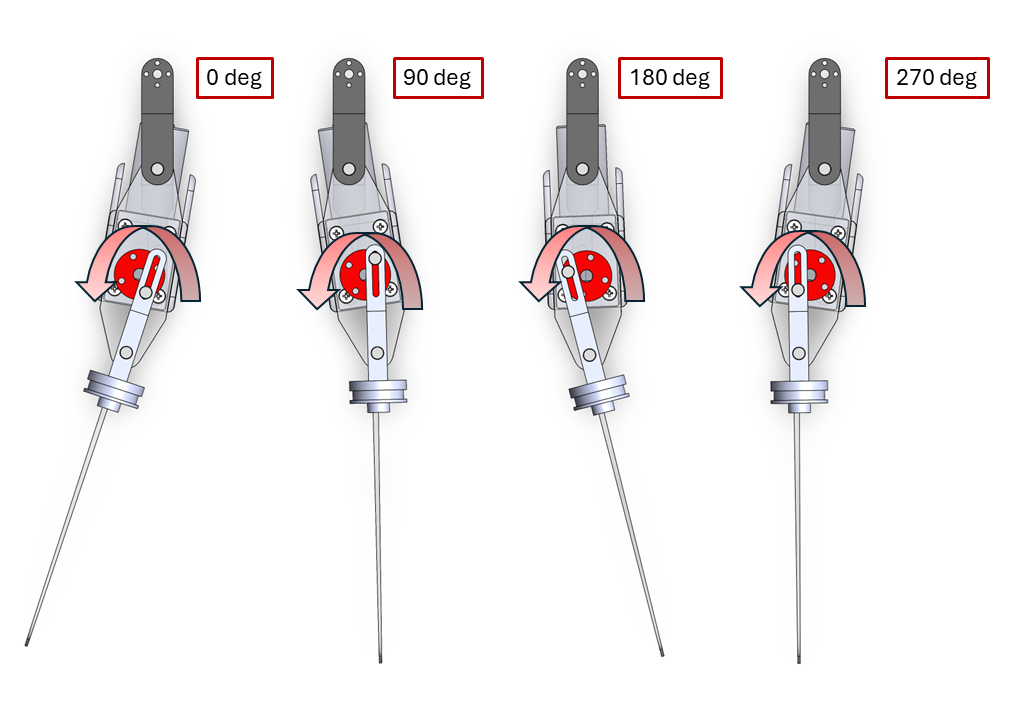
\includegraphics[width=0.9\textwidth]{Fig/DSC-Mech-action.png}
    \caption{The double slider-crank mechanism}\label{DSC_operation}
\end{figure}
\par A servo motor is part of the steering system which orients the complete DSC based tail mechanism, to push the steering/heading angle of the robot. The ground link of the DSC mechanism is connected to the moving shaft of the servo motor while the stator of the servo motor is grounded to the robot's body. The movement of the servo motor with its corresponding movement of the DSC mechanism is shown in the Fig.~\ref{servo_movement}.
\begin{figure}[hpt]
    \centering
    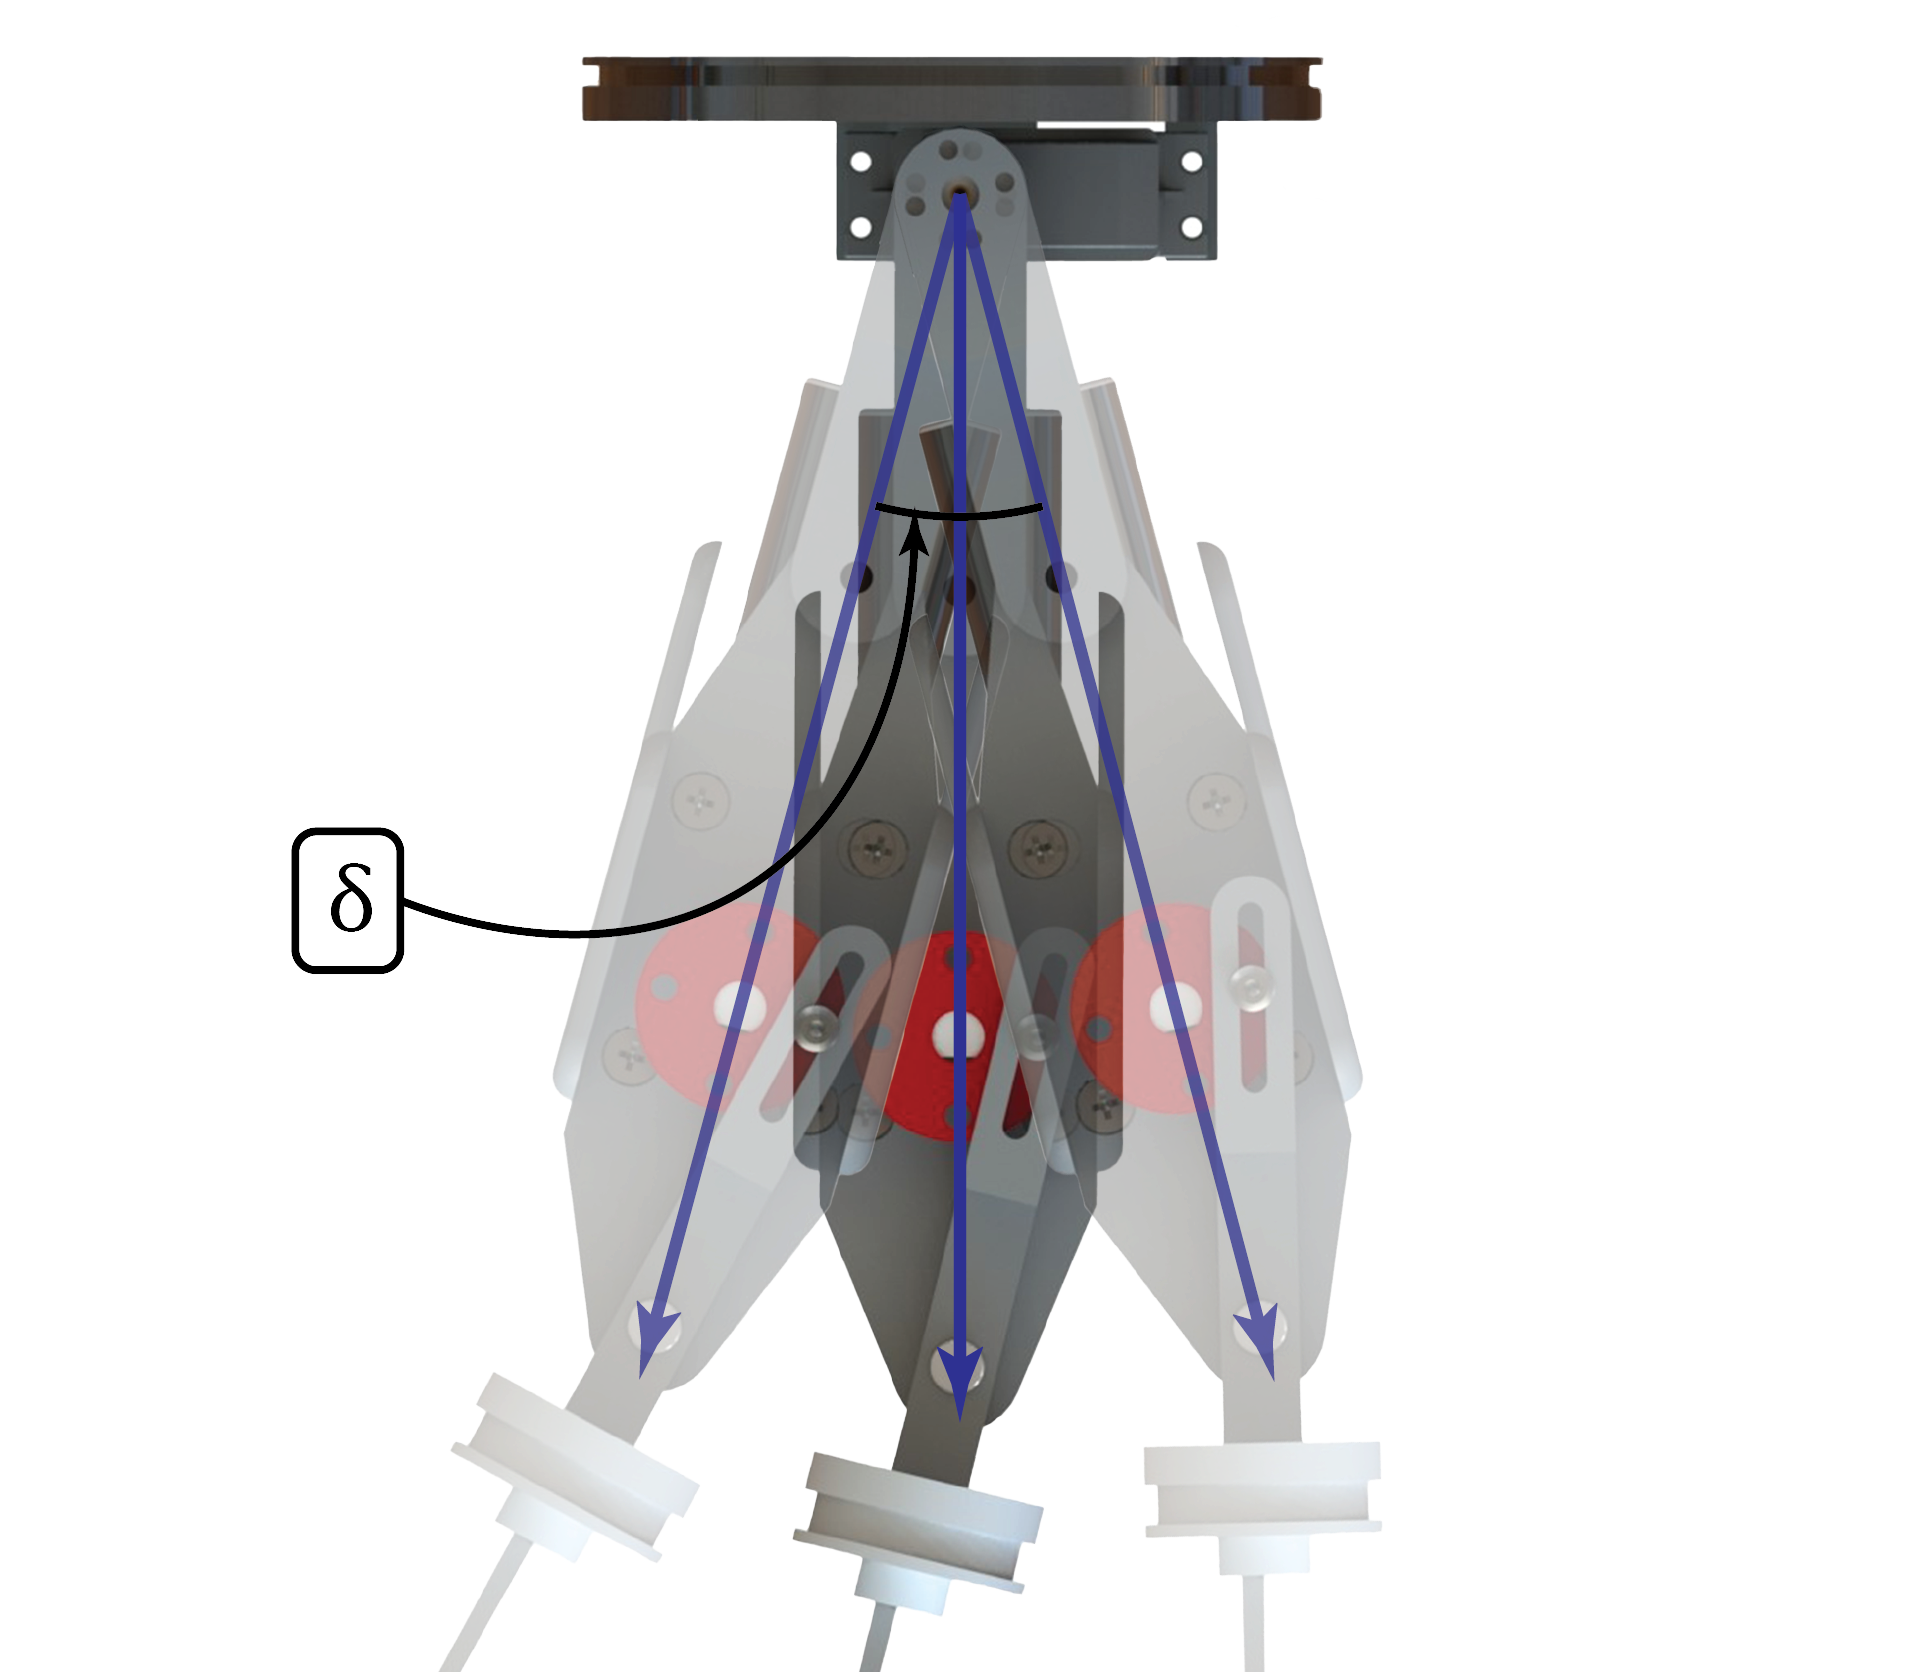
\includegraphics[width=0.6\textwidth]{Fig/Tail_Servo_Movement-01.png}
    \caption{The tail bias angle moving the DSC thrust mechanism}\label{servo_movement}
\end{figure}
\subsection{Electronics Enclosure and Cosmetic Cover}
The AquaNavigator is capable of adjusting depth in static manner. The depth control is achieved through a piston-cylinder based mechanism.The piston-cylinder system is designed to adjust the buoyancy of the robot. The piston is actuated by a linear actuator from Actuonix Motion Devices Inc which provide a linear analog position feedback for precise control. This buoyancy control device is discussed in detail in the previous work of the authors \cite{Masood2023}. The linear actuator is fit into the electronics water tight enclosure so it does not need to have any specific ingress protection. \par
Other than that, an RGB Camera from Sony is also mounted within this enclosure. The camera is placed in the front of the robot, and the cosmetic head of the robot is designed in a way to allow the vision pass through it to the camera. The camera is fixed at a tilt angle of $30\deg$ down from the horizon. A vacuum face seal gland is designed to achieve the ingress protection standard of IP-68 for the watertight enclosure, which is further tested through continuous submersion at $1m$ depth for three days. The penetrators from BlueRobotics\texttrademark{} are used for wiring. Servo motor for the tail angle movement and the DC motor for the double slider-crank mechanism are individually sealed with Loctite Marine Epoxy and can be exposed in water directly. 
The overall design of the robot fish is made ellipsoidal to minimize the drag in the water and maximize the thrust force because of the flapping. The steady state speed of the robot's motion is dependent on the frequency and the constant phase angle in the oscillatory foil motion of the DSC mechanism. In this study, the optimum frequency with a corresponding speed of the robot is maximized with a series of experiments and been fixed for the complete operation during the application.
\begin{figure}[hpt]
    \centering
    \subfloat[]{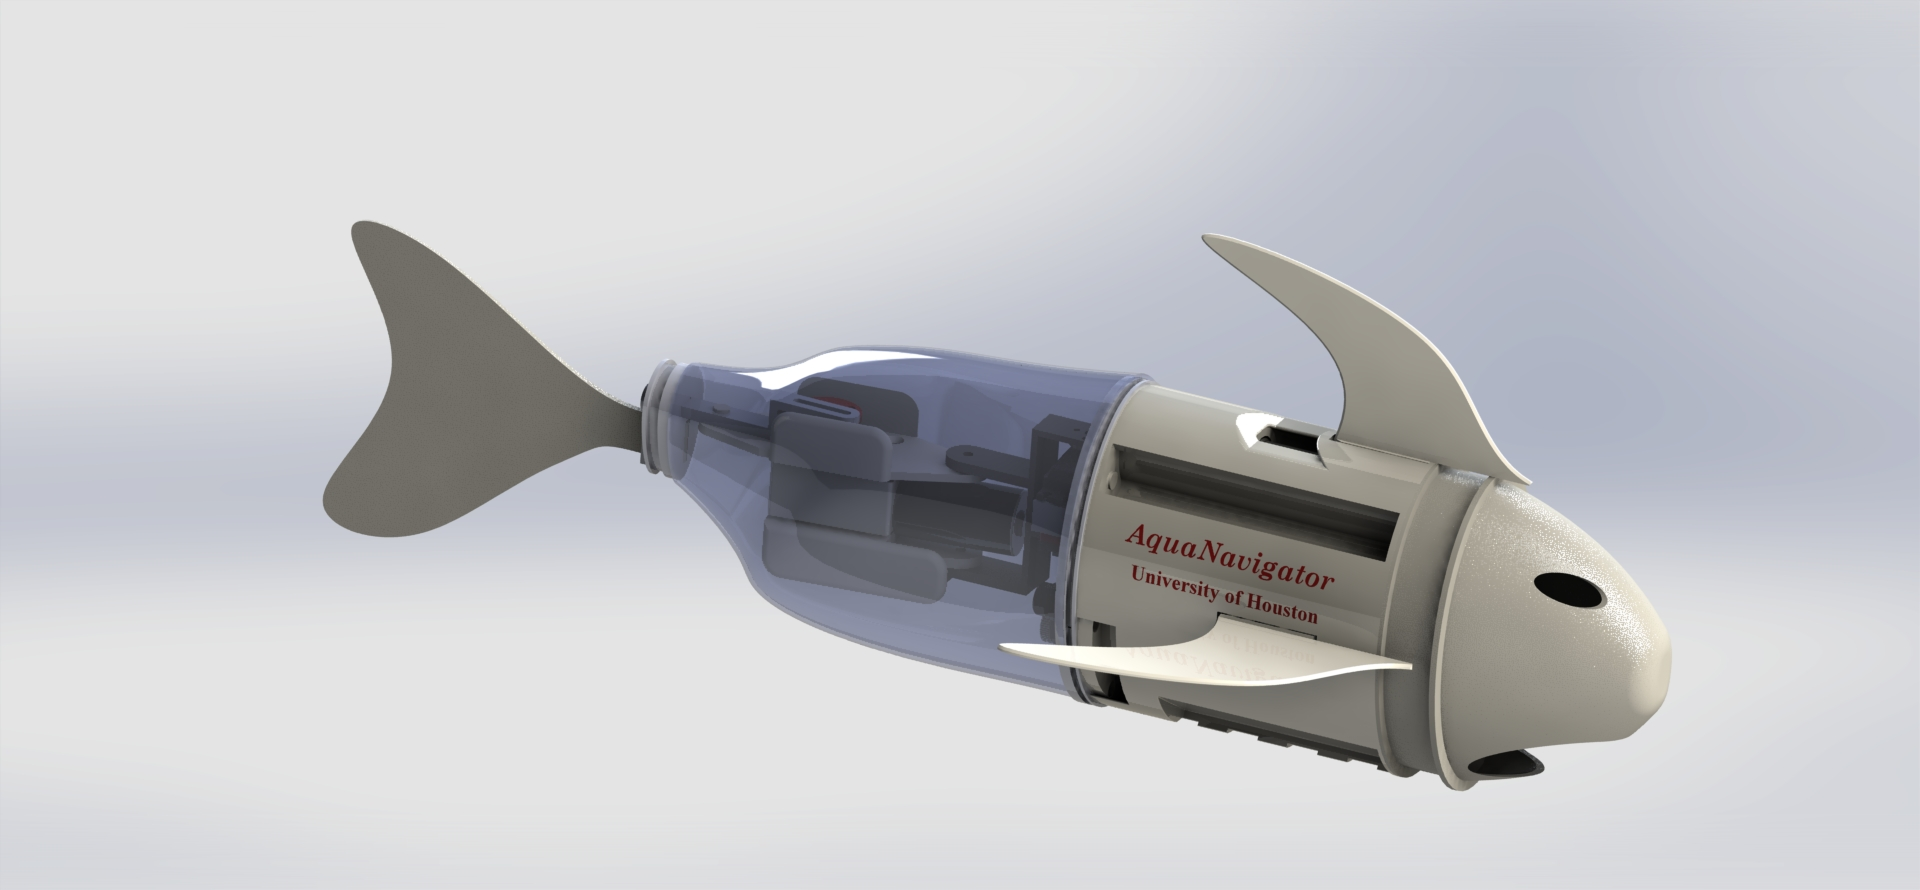
\includegraphics[width = 0.9\textwidth]{Fig/20240627-Fish-SideView.JPG}}
    \vfill
    \subfloat[]{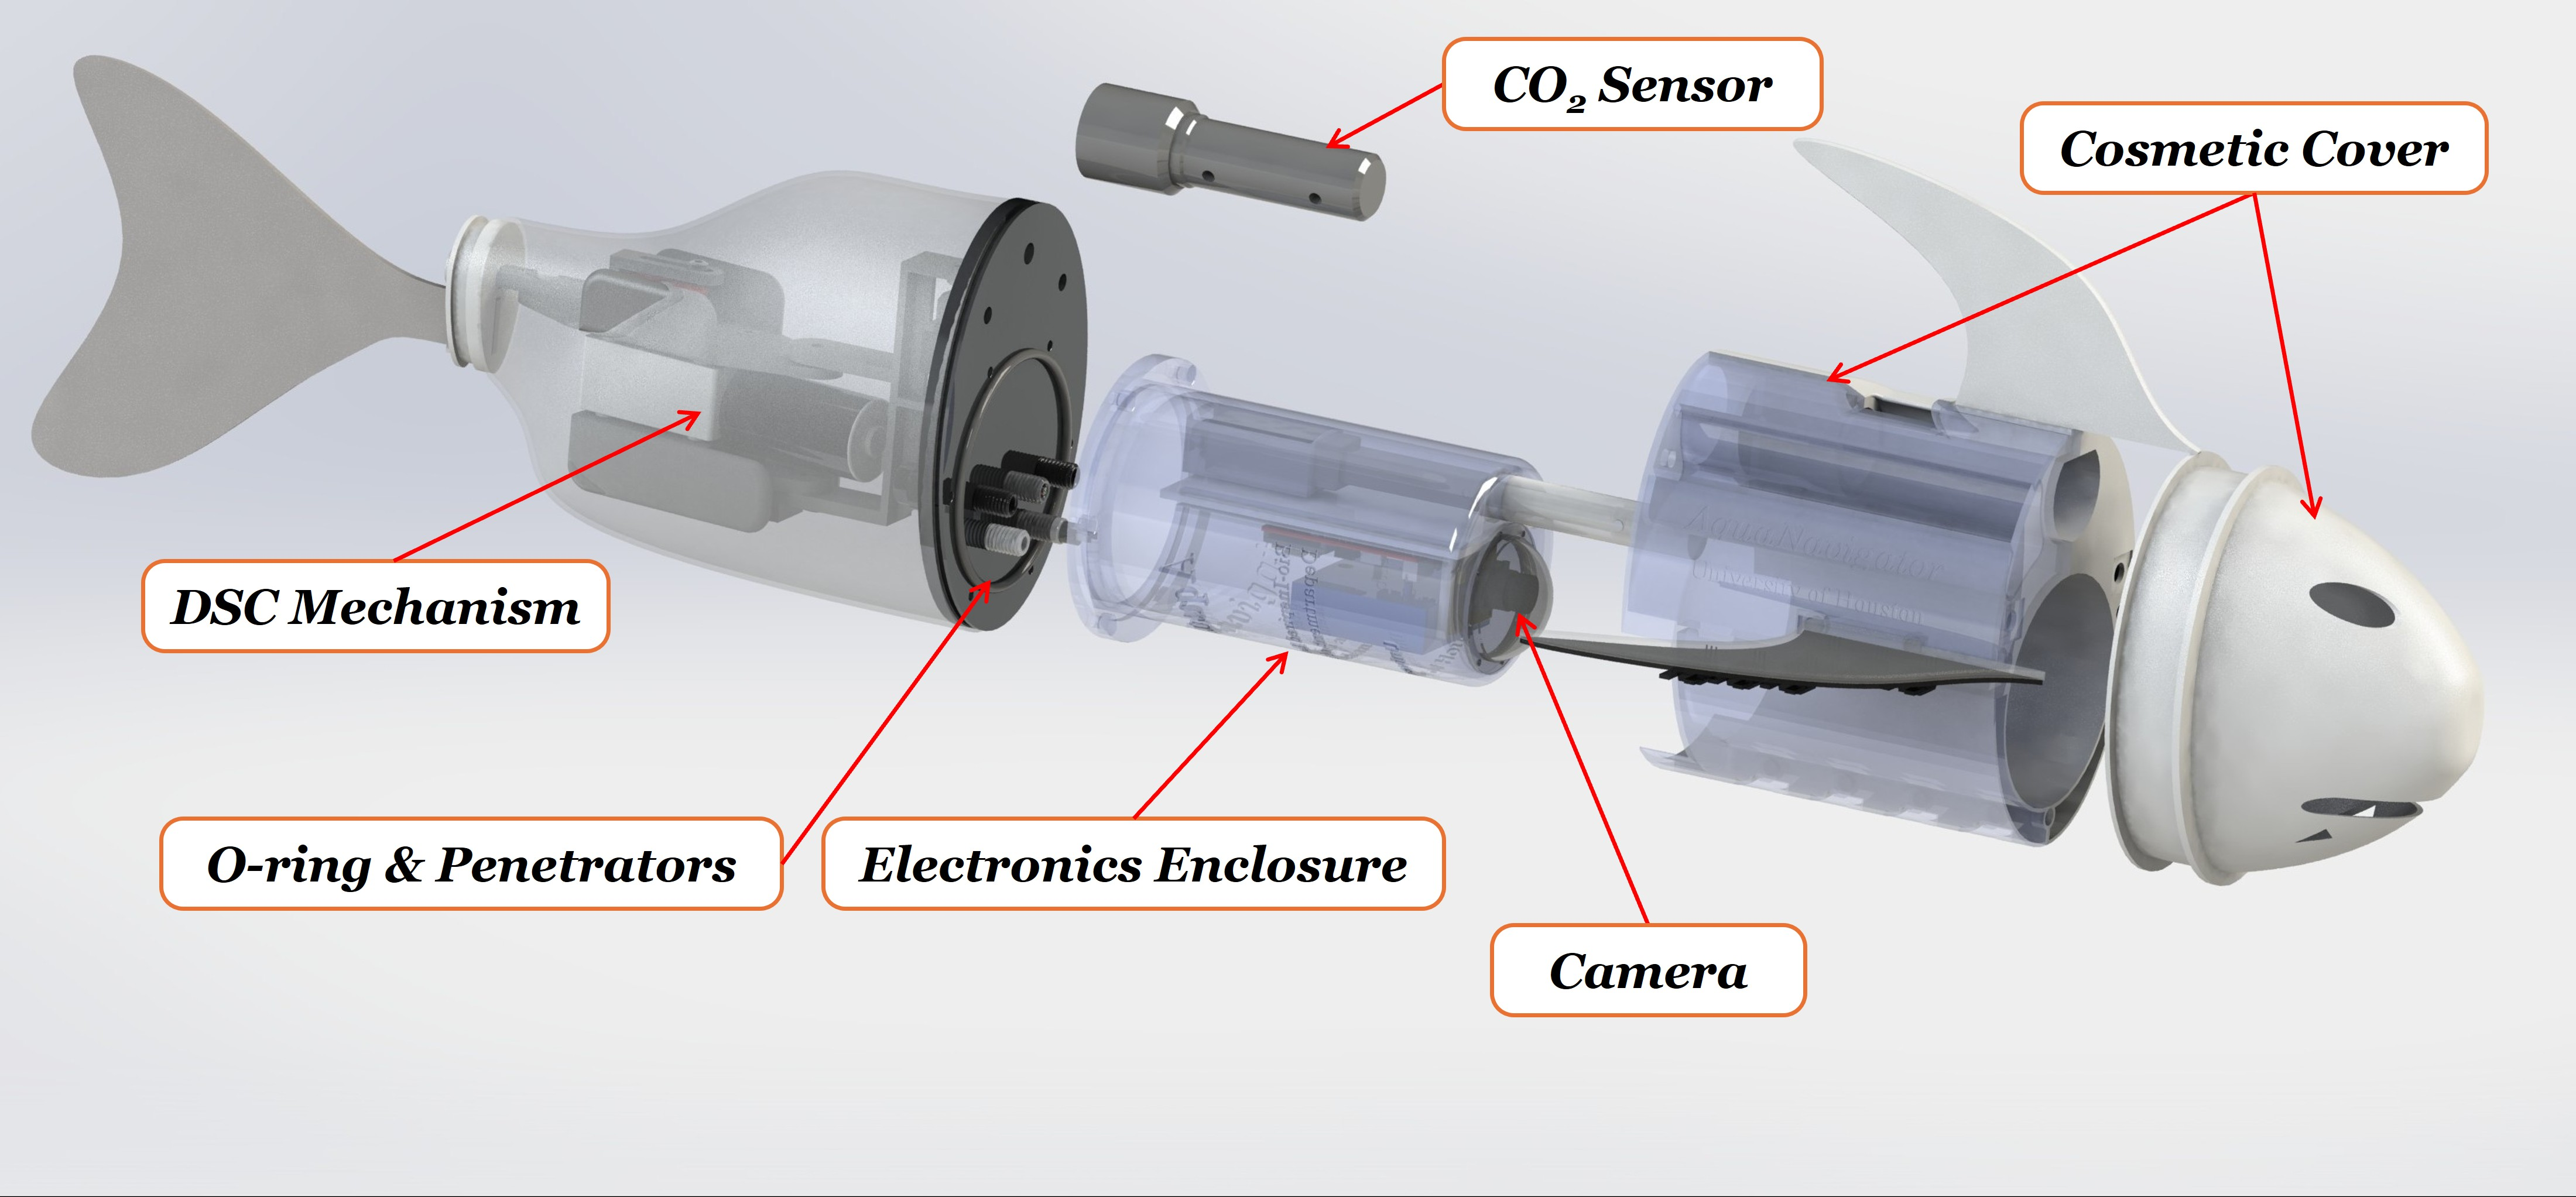
\includegraphics[width = 0.9\textwidth]{Fig/NSF_Exploded_Mirror.JPG}}
    \caption{The complete design of the AquaNavigator in CAD}\label{CAD_AquaNavigator}
\end{figure}
\section{Dynamic Model}\label{modeling}
\par The dynamic model of the robotic fish is derived in two parts (1) Estimation of the force generated by the flapping tail mechanism and (2) 2D planar dynamics of the robots movement on the water surface. In the following paragraphs following frames of reference will be used and shown in the Fig.~\ref{fig:fishframes}. 
\begin{figure}
    \centering
    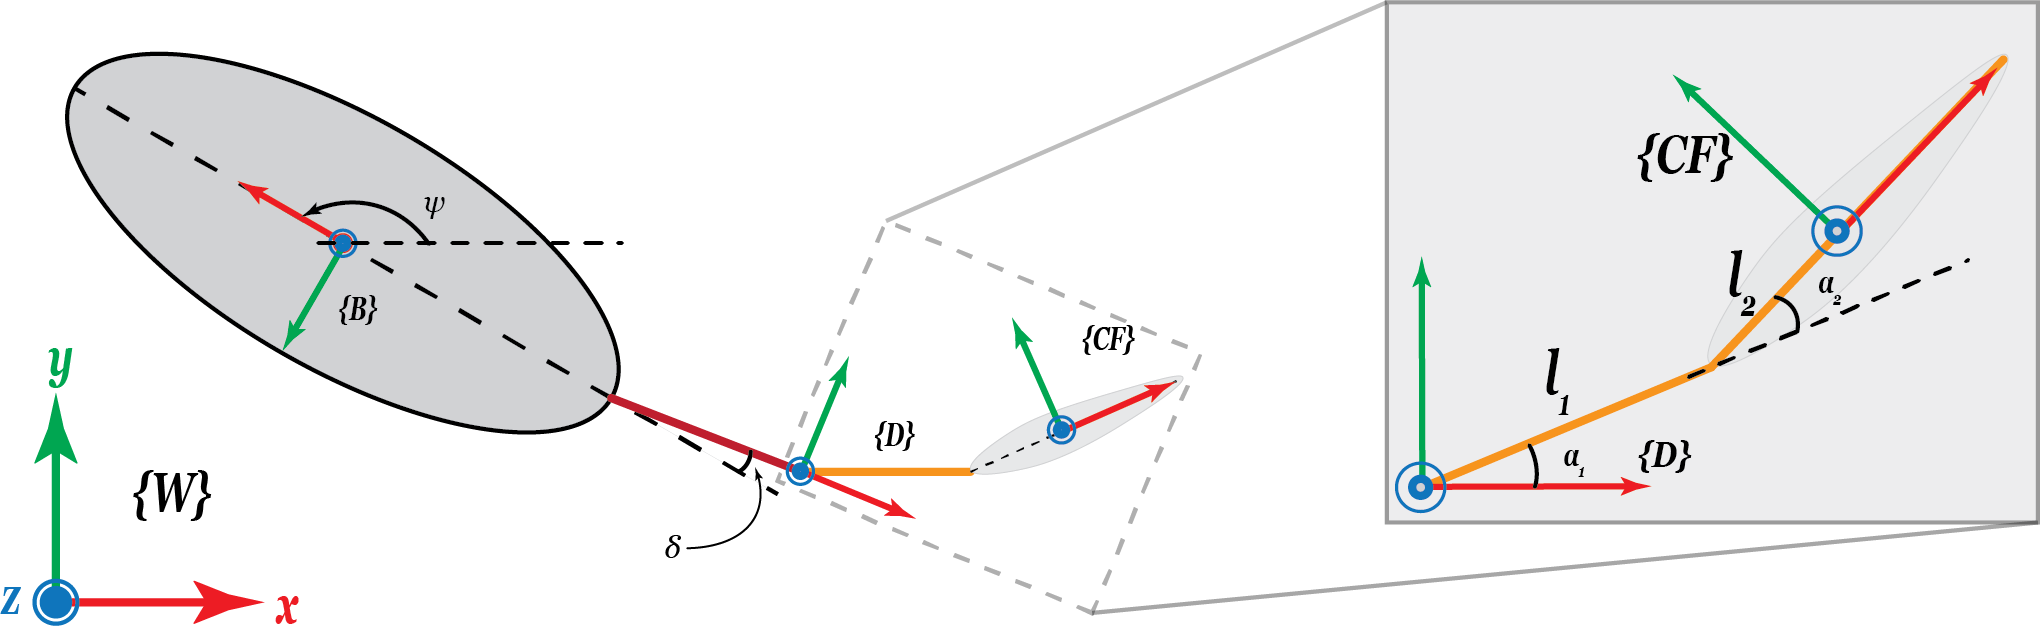
\includegraphics[width=0.9\textwidth]{Fig/RoboticFish-Frames.png}
    \caption{Frames of reference for the robotic fish}
    \label{fig:fishframes}
\end{figure}
\begin{enumerate}
    \item \textbf{World Coordinates Frame $\mathbf{\{W\}}$:} Can be arbitrarily placed anywhere on the water surface, with $z$-axis pointing downwards. The orientation of the $x$ and $y$ axes can be chosen arbitrarily as far as they are orthogonal to each other and following the right-hand rule with sequence $x-y-z$. For most experiments and simulation the origin is placed at the bottom left corner of the water tank in the top camera view.
    \item \textbf{Body Frame $\mathbf{\{B\}}$:} The origin of the body frame is at the center of mass of the robot, with $z$-axis pointing downwards, while $x$ and $y$ axes are aligned with the heading and lateral directions of the robot, respectively. 
    \item \textbf{DSC Frame $\mathbf{\{D\}}$:} The origin of the DSC frame is at the joint between $l_0$ and $l_1$ in the tail. This joint is essentially the origin of the DSC mechanism. The $z$-axis is again downwards, and $x$-axis is aligned with $l_0$.
    \item \textbf{Caudal Fin Frame $\mathbf{\{CF\}}$:} The origin of the caudal fin frame is at the quarter-chord point of the caudal fin, with $z$-axis pointing downwards, while $x$ and $y$ axes are aligned with the normal and tangential directions of the caudal fin, respectively.
\end{enumerate}
\par As the scope of the application in this research work does not extend to the depth control, definition of $z$-axis in the frames about may seem redundant in the coming paragraphs, but they are mentioned for the sake of completeness and consistency in future work. 
\subsection{Hydrodynamic Forces and Thrust Estimation}
\par For dynamic model of the robotic fish operation we closely follow the methodology shown in \cite{Wang2013} with some sort of modification related to the double slider crank mechanism which affect the normal and tangential velocities of the tail end part as compared to simply oscillating rigid foil. Though the double slider crank mechanism is build with rigid links, but it has better tendency to follow a curved path. Anyways, it is important to note at this point, the complex interaction between rigid links and the fluid, and the fluid flow around the moving robotic fish is still to be studied by the researchers. In this regard Lighthill's large-amplitude elongated body theory \cite{Lighthill1971}, gives a close approximation of the fluid-structure interaction and resulting thrust force. The assumptions taken in this work are as follows
\begin{enumerate}
    \item The pitch motion $(q)$ and roll motion $(p)$ are assumed to be constantly zero. This assumption is realized with the fact that the center of the mass of the robot is adjusted in the lower part and exactly in the middle laterally. So the robot will always be aligned to the surface of the fluid keeping pitch $(q)$ and roll $(p)$ to be zero.
    \item The robotic fish is treated as a non-holonomic system due to its underactuated dynamics specifically, the inability to generate independent control in the lateral (sway) direction. Although planar motion is assumed (3 DOF: surge, sway, yaw), the sway motion results from hydrodynamic interactions rather than direct actuation. This non-holonomic constraint is typical in mobile robots with drift and is considered in the design and selection of control algorithms.
    \item The body-fixed coordinate system consists of heading velocity $(u)$, heave velocity $(v)$, and yaw motion $(r)$, which coincides with the center of mass of the robotic fish. This simplifies the analysis by aligning the steering of the robotic fish with respect to the z-axis in the body-fixed coordinate system.
    \item The fluid surrounding the robotic fish is considered to be inviscid which implies the viscous resistance on the robot's body can be ignored. This simplification is common in theoretical fluid dynamics models to focus on the effects of pressure and inertial forces.
    \item In the context of elongated body theory (EBT) and the assumption of a quasi-steady state for the caudal fin, it is assumed that the fluid-structure interaction is minimized due to the high stiffness of the fin and low-frequency oscillations. 
\end{enumerate}
\par The movement of the caudal fin is generated by the double slider crank mechanism. The amplitude of each of the links' rotary motion range is denoted as $A_1$ and $A_2$ and at a phase difference of $\phi_{dsc}$. When the DSC is operated at a speed of $\omega$ the instantaneous angular position of each link of DSC is:
\begin{equation}
    \begin{aligned}
        \alpha_1(t) &= A_1 \sin(\omega t), \\
        \alpha_2(t) &= A_2 \sin(\omega t + \phi_{dsc}).
    \end{aligned}
\end{equation}
The phase difference $\phi_{dsc}$ is estimated to perform the best at $\pi/2~rad$ in the literature \cite{Zuo2021} so for the sake of simplicity further derivation is shown for fixed phase difference. The position and velocities at the quarter-chord point of the caudal fin are given in the $\{D\}$ frame as:
\begin{equation}
    \begin{aligned}
        x_{qc} &= l_1 \cos(\alpha_1) + l_2 \cos(\alpha_2), \\
        y_{qc} &= l_1 \sin(\alpha_1) + l_2 \sin(\alpha_2), \\
        \dot{x_{qc}} &= -l_1 \omega \sin(\alpha_1) - l_2 \omega \sin(\alpha_2), \\
        \dot{y_{qc}} &= l_1 \omega \cos(\alpha_1) + l_2 \omega \cos(\alpha_2),
    \end{aligned}
\end{equation}
where $l_1$ and $2l_2$ are the lengths of the links of the DSC mechanism, and shown in Figure.~\ref{DSC_operation}. The velocities of the quarter-chord point in ${CF}$ frame, which can also be regarded as normal and tangential velocities, are given as:
\begin{equation}
    \begin{aligned}
        V_\parallel &= - \dot{x_{qc}} \sin(\alpha_2) + \dot{y_{qc}} \cos(\alpha_2),  \\
        V_\perp  &= \dot{x_{qc}} \cos(\alpha_2) + \dot{y_{qc}} \sin(\alpha_2).
    \end{aligned}
\end{equation}
\par The elongated-body theory (EBT) is used to estimate the thrust force generated by the caudal fin. The thrust force in the $\{D\}$ frame is given as:
\begin{equation}
    {}^{D}F = \frac{1}{2} m_i V_\perp^2 \hat{m} - m_i V_\perp V_\parallel \hat{n} + m_i L \dot{V_\perp} \hat{n}.
\end{equation}
The bias angle of the tail is denoted as $\delta$ and the force generated by the tail is transformed to the body frame as
\begin{equation}
    {}^{B}F = 
    \begin{bmatrix}
        F_x \\
        F_y
    \end{bmatrix}
    =
    \begin{bmatrix} 
        \cos(\delta) & -\sin(\delta) 
        \\ \sin(\delta) & \cos(\delta) 
    \end{bmatrix} 
    {}^{D}F,
    \label{eq:fxy}
\end{equation}
where, $m_i = \frac{1}{4} \pi \rho_w h^2$ denotes the virtual mass per unit length where $\rho_w$ is the density of the fluid and $h$ is the height of the robotic fish in the water. $L = 2d_0 + l_0 + l_1 + l_2$ is the complete length of the body. Then the moment in the robot can be written as:
\begin{equation}
    F_{\theta} = - \left( (L - d_0) \cos(\delta) \right) F_y + (l_0 + l_1 + l_2) \sin(\delta) F_x,
    \label{eq:theta}
\end{equation}
where $L = 2d_0 + l_0 + l_1 + 2l_2$ is the complete length of the body. Above is the thrust force generated by the caudal fin with the DSC mechanism operating at a frequency $\omega$ and a bias angle $\delta$, where $\omega$ has units of $rads^{-1}$. 
\subsection{Rigid Body Dynamics}
Thrust force and moments are calculated in Eq. \ref{eq:fxy} and Eq. \ref{eq:theta} respectively. The forces acting on the robot are the thrust force generated by the caudal fin, the drag force acting on the robot, and inertia is caused by the mass as well as the added mass of the fluid flow. Generalized equations of motion for a surface swimming vessel are given as:
\begin{equation}
    \textbf{M}\dot{\nu} + \textbf{C}(\nu)\nu + \textbf{D}\nu = \textbf{F},
\end{equation}
where $\nu = [u, v, r]^T$ is the velocity vector of the robot in the body-fixed frame, $\textbf{M}$ is the mass matrix, $\textbf{C}(\nu)$ is the Coriolis matrix, $\textbf{D}$ is the damping matrix, and $\textbf{F}$ is the force vector acting on the robot. The equations of motion of the robotic fish are given as:
\begin{equation}
    \begin{matrix}
        F_x + (m + k_{22}m)vr - D_u u - (m + k_{11}m)\dot{u} = 0, \\
        F_y + (m + k_{11}m)ur - D_v v - (m + k_{22}m)\dot{v} = 0, \\
        F_\theta - (k_{22}m - k_{11}m)uv - D_r r - (I + k_{55}I) \dot{r} = 0,
        \label{eq:eom}
    \end{matrix}
\end{equation}
where $m$ is the mass of the robot, $I$ is the moment of inertia of the robot, $k_{11}$, $k_{22}$, and $k_{55}$ are the added mass coefficients in the $u$, $v$, and $r$ directions, respectively. $D_u$, $D_v$, and $D_r$ are the drag coefficients in the $u$, $v$, and $r$ directions, respectively. The added mass coefficients are calculated with an assumption that the robotic fish is a prolate ellipsoid with semi-axis $a$, $b$, and $b$ in the $x$, $y$, and $z$ directions, respectively. Lamb's $k$-factors representation is used to calculate the added mass coefficients as follows:
\begin{equation}
    \begin{aligned}
        k_{11} &= \frac{\alpha_0}{2 - \alpha_0}, \\
        k_{22} &= \frac{\beta_0}{2 - \beta_0}, \\
        k_{55} &= \frac{e^4(\beta_0 - \alpha_0)}{(2-e^2)(2e^2 -(2-e^2)(\beta_0 - \alpha_0))},
    \end{aligned}
\end{equation}
where,
\begin{equation*}
    \begin{aligned}
        \alpha_0 &= \frac{2(1-e^2)}{e^3} \left( \frac{1}{2} \ln \frac{1+e}{1-e} - e \right),\\
        \beta_0 &= \frac{1}{e^2} - \frac{1 - e^2}{2e^3} \ln \frac{1+e}{1-e}
    \end{aligned}
\end{equation*}
and $e = \sqrt{1 - \frac{b^2}{a^2}}$ is the eccentricity of the ellipsoid.
\par The added mass approximations above are very critical in the modeling as they directly impact the inertia considered for the rigid body dynamics. It is important to note that the Lamb's k-factors are calculated with an assumption that the body of the robotic fish is a prolate ellipsoid with mass $m$ and moment of inertia $I$. So this lead us to use the most accurate values of the semi-axes of the ellipsoid to by keeping the following relationship true:
\begin{equation}
    m = \frac{4}{3} \pi \rho_w ab^2,
    I = \frac{4}{15} \pi \rho_w ab^2 (a^2 + b^2).
\end{equation}
It is important to note here that the robotic fish is carefully estimated to be a prolate ellipsoid, and special has to be paid when estimating size of the ellipsoid which gives the closest approximation in terms of mass, density, and moment of inertia. For the specific prototype of the AquaNavigator, and may be any other robotic fish developed until now, the density of the robot outside the water and inside the water is not same, considering any pores in the body. Usually when measuring the mass of the robot, we consider the mass outside the water and it doesn't include any cavities or the pores in the structure. Though the overall density of this robot will still be the same and density of water $\rho_w$ but the mass or inertia properties will be different. For example, in the specific case of the AquaNavigator, there has been some designed hollow and water filled cavities, in the cosmetic cover and the tail part, which will be filled with water when the robot is in operation. This has to be considered when estimating $a$ and $b$ for the ellipsoid. For the purpose of the added mass, what matters the most is the over all size, and the mass to be accurately estimated. Knowing the size of the robot, $a$ and $b$ are estimated to cover the the complete robot without the caudal fin in the end. The effective mass of the robot can be calculated from the fact that the density of the overall robot in water is same as $\rho_w$. The values are mentioned in Table \ref{tab:exp_vals}.
\par The other important parameter in the Eq. \ref{eq:eom} is the uncoupled damping coefficients $D_u$, $D_v$, and $D_r$. The hydrodynamic drag on the rigid body has many shapes including but not limited to; (1) radiation-induced potential damping, (2) linear skin friction, (3) wave drift damping and (4) damping due to vortex shedding. All of these damping forces are highly non-linear and coupled in nature. Nevertheless, on rough approximation could be to assume that (1) the underwater robot is performing a non-coupled motion, (2) lumped damping coefficient takes into consideration all the damping forces, and (3) the terms higher than second order are negligible. The damping coefficients are as follows:
\begin{equation}
    \mathbf{{D}} =
    \begin{bmatrix}
        D_u & 0 & 0 \\
        0 & D_v & 0 \\
        0 & 0 & D_r
    \end{bmatrix} =
    \begin{bmatrix}
        \frac{\delta F_x}{\delta u} & 0 & 0 \\
        0 & \frac{\delta F_y}{\delta v} & 0 \\
        0 & 0 & \frac{\delta F_\theta}{\delta r}.
    \end{bmatrix}
\end{equation}
An estimation for the damping coefficient can be found empirically through a series of experiments in a water tank or by the hydrodynamic derivatives as, partial derivative of the drag forces with respect to the velocity components. The drag forces acting on the robot are given as:
\begin{equation*}
    \begin{aligned}
        F_{D_u} &= \frac{1}{2} \rho_w A_u C_u |u| u, 
        F_{D_v} = \frac{1}{2} \rho_w A_v C_v |v| v, 
        F_{D_r} &= C_r |r| r,
    \end{aligned}
\end{equation*}
where, $A_u$, $A_v$, and $A_r$ are the cross-sectional areas of the robot in the $u$, $v$, and $r$ directions, respectively, and $C_u$, $C_v$, and $C_r$ are the drag coefficients in the $u$, $v$, and $r$ directions, respectively. Either these can be used as non-linear damping coefficients in the model or a linear approximation can be used as in the following equation:
\begin{equation*}
    \begin{aligned}
        D_{u}(\bar{u}) &= \left. \frac{\delta D_u}{\delta u} \right|_{u = \bar{u}}, 
        D_{v}(\bar{v}) = \left. \frac{\delta D_v}{\delta v} \right|_{v = \bar{v}},
        D_{r}(\bar{r}) &= \left. \frac{\delta D_r}{\delta r} \right|_{r = \bar{r}}.
    \end{aligned}
\end{equation*}
\par The drag coefficients can be found for standard shapes as ellipsoid in literature and the values are mentioned in the Table.~\ref{tab:exp_vals}. The dynamic model of the robotic fish is given in Eq.~\ref{eq:eom} and the drag coefficients are given in Table \ref{tab:exp_vals}. The model is used to simulate the motion of the robotic fish in the water tank and to design a control algorithm for the robotic fish.
\begin{table}[ht]
    \centering
    \begin{tabular}[width=\linewidth]{ccc}
        \toprule
        Parameter & Value & Unit \\
        \midrule
        \multicolumn{3}{c}{Experimental Values} \\
        \midrule
        $C_u$ & 0.05 & $kg/s$ \\
        $C_v$ & 18.5 & $kg/s$ \\
        $C_r$ & 0.49 & $kg/s$ \\
        $k_f$ & 0.45 & N/A \\
        \midrule
        \multicolumn{3}{c}{Calculated Values} \\
        \midrule
        $a$ & 0.234 & m \\
        $b$ & 0.065 & m \\
        $e$ & 0.96 & \\
        $\alpha_0$ & 0.173 & \\
        $\beta_0$ & 0.9135 & \\
        $k_{11}$ & 0.0947 & \\
        $k_{22}$ & 0.8408 & \\
        $k_{55}$ & 0.5587 & \\

        \midrule
        \multicolumn{3}{c}{Geometric and Body Parameters} \\
        \midrule
        $m_e$ & 4.14 & kg \\
        $I$ & 0.049 & kg m$^2$ \\
        $l_0$ & 0.06 & m \\
        $l_1$ & 0.1176 & m \\
        $l_2$ & 0.097 & m \\
        $d_0$ & 0.145 & m \\
        $A_1$ & 10 & deg \\
        $A_2$ & 13 & deg \\
        $\phi_{dsc}$ & 90 & deg \\
        \bottomrule
        \vspace{1em}
    \end{tabular}
    \caption{Experimental and Calculated Values of the Parameters}
    \label{tab:exp_vals}
\end{table}
\section{Robotic Fish Simulator}
\par To facilitate dynamic model parameter estimation, model validation, and control design, a modular simulator environment was developed. This simulator enables efficient tuning of control gains, regardless of whether a model-based or model-free control strategy is employed. This section focuses primarily on the architecture and design of the simulator, which comprises key components such as the robotic fish, the water tank, and the pipelines. To maintain generality and modularity, implementation-specific parameters—such as time steps, control loop frequencies, or object dimensions—are intentionally omitted in this section and are instead discussed alongside the results where relevant. 
\subsection{Simulator Design}
\par The dynamic model developed in Eq. \ref{eq:eom} and all the preceding equations are solved in numerical discrete time simulation with fixed time stepping. Python library SciPy \cite{2020SciPyNMeth} is employed for the numerical solutions through the $\mathtt{solve\_ivp}$ function. This function uses the Runge-Kutta 45 method to solve the initial value problem (IVP) for the system of ordinary differential equations (ODEs) derived from the dynamic model. Further details on the numerical solution and convergence can be found in the documentation of the SciPy library. The simulator is designed with future extensibility in mind, supporting not only ongoing research within this lab but also contributions from the broader research community interested in underwater robotics. It adopts an object-oriented architecture, featuring a generic robot class capable of simulating any underwater robot that utilizes tail-based propulsion. Implemented in Python, the simulator emphasizes reusability and modularity. The simulator has been validated using the AquaNavigator platform, with performance results presented in the subsequent sections.\par
Furthermore, for the purpose of this study, classes for water tank and pipes are also developed in the simulator. The 3D rendering is done using the $\mathtt{vpython}$ module which allows to be visualized on a web browser during the runtime, and can also be rendered as a video file. Fish object maintains the history of multiple data points (some states and control signals) which can be retrieved in the end of the simulation to show on a plot or store in a $\mathtt{.csv}$ file, during the control design study or open-loop dynamic model validation. 
\par All geometric parameters of the robotic fish are defined as class attributes, whereas the fluid interaction parameters are kept local to the Initial Value Problem (IVP) solution function, as they depend on specific operating conditions and are not intrinsic properties of the robotic fish. Future improvements to the simulator are under consideration to further mature it into a unified platform that can support the development and testing of advanced control techniques for underwater robotics. While the simulator plays an important supporting role in this work, it is not the primary contribution of the research. The overall structure of the simulator is illustrated in Algorithm~\ref{alg:simulator}.
% algorithm table
\begin{algorithm}[H]
    \caption{Simulator Algorithm}
    \label{alg:simulator}
    \begin{algorithmic}[1]
        \STATE Initialize the robotic fish position, orientation and shape
        \STATE Initialize constant tail beat frequency $\omega = \omega_0$
        \STATE Initialize the water tank and pipeline dimensions
        \STATE Initialize simulation parameters $t_0$, $t_f$, $\Delta t$
        \STATE Compute number of steps $N = \frac{t_f - t_0}{\Delta t}$
        \STATE Initialize $t_0 = 0$, $y_0$, arrays for $t$ and $y$
        \FOR{$n = 0$ to $N-1$}
            \STATE Compute $t_{n+1} = t_n + \Delta t$
            \STATE \textbf{Control:} Compute the control signal $\delta$ as using the visual servoing
            \STATE Compute tail deflection angles $\alpha_1(t_n)$, $\alpha_2(t_n)$
            \STATE Compute tail-tip coordinates and velocities: $x_{qc}, y_{qc}, \dot{x}_{qc}, \dot{y}_{qc}$
            \STATE Compute parallel and perpendicular velocities: $V_\parallel$, $V_\perp$
            \STATE Compute hydrodynamic forces and moment: $F_x, F_y, F_\theta$
            \STATE \textbf{Runge-Kutta 45 Solver:}
            \STATE \hspace{1em} Use current state as initial condition
            \STATE \hspace{1em} Solve Eq.~\ref{eq:eom} for updated states $u_{n+1}, v_{n+1}, r_{n+1}$
            \STATE Compute position and orientation updates: $x$, $y$, $\psi$
            \STATE Update and store the state of the robotic fish
        \ENDFOR
        \STATE Plot simulation results
    \end{algorithmic}
\end{algorithm}
\section{Image Processing and Visual-Servo Control}\label{Visual_servoing}
\par This section describes the image processing and visual-servoing control of AquaNavigator. Without using any sonar or underwater localization sensors, AquaNavigator purely uses its onboard camera for pipeline tracking. The challenges come from pipeline detection and control of under-actuated dynamics. In this section, a Hough transformation-based image processing is developed for pipeline detection. Then a unique control with a single tracking angle as the input is developed to control AquaNavigator to converge both heading direction and position respective to the detected pipeline to zero. 
\subsection{Pipeline Detection}
\par The camera is mounted in the front of the fish within the circuitry enclosure which keeps it safe from the water but through a transparent dome, it can still see the surroundings as an RGB image. The cosmetic head of the fish is designed in a way to allows the vision to pass through it to the camera. Fig.~\ref{fig:pipeline_tracking_POV} shows the view of the camera from the robotic fish and seeing the pipeline. The tilt angle of the camera is fixed and designed with iterative experimentation, and set to $30~\deg$ down from the horizon. The image from the CMOS camera is transmitted through a Universal Serial Bus (USB) to the host computer where the image is processed in a Python-based program utilizing OpenCV functions.
\par The Canny Edge Detection algorithm is used to detect the edges in the frame, followed by necessary cropping and light enhancements in the image. Hough Algorithm then combines the edges and creates complete probable lines, where the most dominant line is the pipeline. As opposed to Position-based Visual Servoing (PBVS), Image-based Visual Servoing (IBVS) is more robust towards any uncertainties in the camera intrinsic, and 3D localization of the pipeline in world coordinates is not necessary. Rather the focus is to transform everything to the 2D Image Space and drive the robot to minimum error in the position and orientation of the robot with respect to the pipeline in the image space. The control algorithm is inspired by Reynolds {\it et al.}\cite{Reynolds1999} and has been adjusted to the typical application in the robotic fish.
\begin{figure}
    \centering
    \includegraphics[width = 0.9\textwidth]{Fig/Control-Scheme-Fish-Pipeline-01.png}
    \caption{Control Scheme for the pipeline tracking}\label{control_scheme}
\end{figure}
\subsection{Visual Servoing Control}
\par For the application in the pipeline tracking visual serving control is one robust method with the camera mounted on the robotic fish. The comparison between image-based or position-based visual servoing has always been in literature but for this specific application it is intended to show the major trade-offs when selecting each one of them. In this regard, the developed simulator would also be of key importance. In preceding paragraphs, we will use the simulation environment to see the performance of the visual servoing control in both image-based and position-based scenarios.
\subsubsection{Position-Based Visual Servoing}
\par From the simulation perspective, the Position-based Visual Servoing (PBVS) is simpler and more straightforward to implement, reason being the absolute position of the robotic fish and the pipeline is always know in the world coordinates. The control signal is calculated in process shown in preceding paragraph. 
\par Consider the detected pipeline is starting from ${}^W\mathbf{p}_{start}$ and ending at ${}^W\mathbf{p}_{end}$. The pipeline vector would be: 
\begin{equation*}
    {}^W\mathbf{P} = {}^W\mathbf{p}_{end} - {}^W\mathbf{p}_{start}.
\end{equation*}
In the case of a simulator, the position of the robotic fish is always known in the world coordinates as ${}^W\mathbf{p}_{fish} = (x,y,0)$ and heading direction $\psi$ from the $x$-axis. The heading direction of the robotic fish can be represented by vector,
\begin{equation*}
    \hat{\mathbf{h}} = [\cos(\psi), \sin(\psi), 0].
\end{equation*}
The magnitude $\|\mathbf{h}\|$ can be arbitrarily selected depending upon how aggressive the control move is required. Though the pipeline is on the bottom surface of the water tank and the robotic fish is always on the surface, consider dropping a projection of the pipeline on the surface. This way we are solving a 2D problem in the $x-y$ plane of world coordinate frame $\mathbf{\{W\}}$ as follows. Drop a normal vector from the $\mathbf{h_{end}}$ to $\mathbf{P}$, 
\begin{equation*}
    \begin{aligned}
        \mathbf{p}_{proj} &= \frac{\mathbf{h_{end} - p_{start}} \cdot \mathbf{P}}{\|\mathbf{P}\|} \mathbf{P}, \\
        \mathbf{P}_{\parallel} &= \mathbf{p}_{proj} - \mathbf{p}_{start}, \\
        \mathbf{y} = \mathbf{P_{\perp}} &=  \mathbf{P}_{proj} - \mathbf{h_{end}}.
    \end{aligned}
\end{equation*}
The point of normal projection on the pipeline will be $\mathbf{p}_{proj}$. Though the angle between the heading direction of the robotic fish and the pipeline is $\psi_p = \cos^{-1} \left( \frac{\mathbf{P}_{\parallel} \cdot \hat{\mathbf{h}}}{\|\mathbf{P}_{\parallel}\| \|\hat{\mathbf{h}}\|} \right)$, the angle between the heading vector and the $\mathbf{p}_{proj}$ is of interest, as this would eliminate the error in position as well as the orientation of the robotic fish with respect to pipeline in $x-y$ plane. This angle is denoted as $\psi_e$ and is calculated as:
\begin{equation}
    \psi_e = \cos^{-1} \left( \frac{\mathbf{(h - y)} \cdot \hat{\mathbf{h}}}{\|\mathbf{h - y}\| \|\hat{\mathbf{h}}\|} \right).
\end{equation}
Converging $\psi_e$ to zero would mean the robotic fish is aligned and positioned with the pipeline in the $x-y$ plane. The control technique will be discussed in the coming sections.
\subsubsection{Image-Based Visual Servoing}
\par In the case of simulator, the position of the robotic fish and the pipeline is always known in the world coordinates. In real-world scenario the situation is different, as the absolute position of the robotic fish and the pipeline is not known. Similarly, in the case of simulator, the image based visual servoing is a challenge as we know the absolute positions but not the image space data. As a first step, we will implement image-based visual servoing in the simulator, for which the real-world positions and orientations will be transformed to the image space. Then, the reverse problem of transforming the image space data to the world coordinates can be used to implement the position-based visual servoing in the real-world scenario.
\par Following frames of reference (Fig.~\ref{fig:worldcameraframes}) will be mentioned in following paragraphs:
\begin{enumerate}
    \item \textbf{World Coordinates Frame $\mathbf{\{W\}}$:} The same as mentioned in the dynamic model section, now the origin is placed at the bottom left corner of the water tank when viewed from the top camera. The $x$ and $y$ axes are aligned with the length and width of the water tank, respectively.
    \item \textbf{Camera Frame $\mathbf{\{C\}}$:} The origin of the camera frame is at the center of the camera lens, with $z$-axis pointing focal axis of the camera, while $x$ and $y$ axes are aligned with the width and height of the image frame, respectively.
    \item \textbf{Image Frame $\mathbf{\{I\}}$:} The origin of the image frame is at the top left corner of the image, with $x$ and $y$ axes aligned with the width and height of the image, respectively. This frame does not have a third axis.
\end{enumerate}
\begin{figure}[ht]
    \centering
    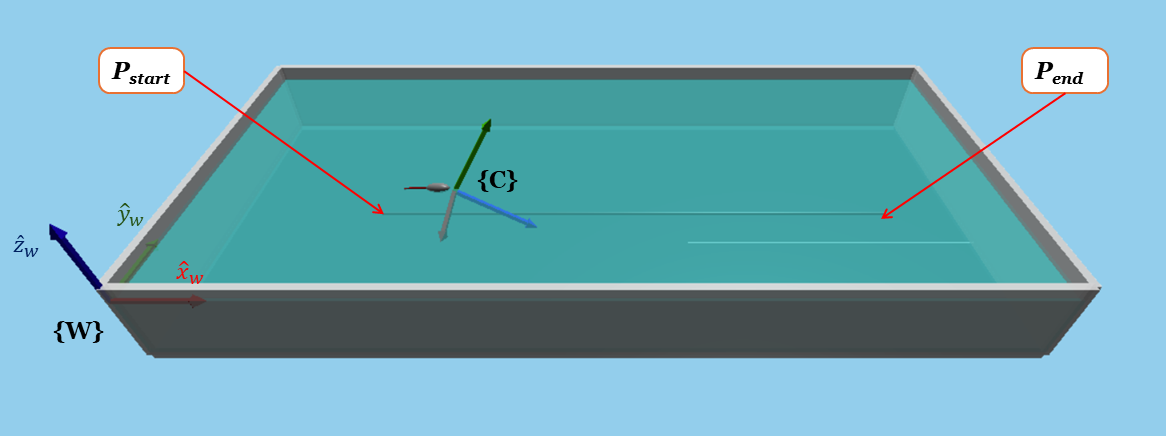
\includegraphics[width = 0.9\textwidth]{Fig/VisualServoing-Frames.png}
    \caption{World and Camera Frames of Reference}
    \label{fig:worldcameraframes}
\end{figure}
\par From the fixed geometry of the robotic fish, the position and orientation of the camera with respect to the center of mass of the robotic fish also known as ${}_W\mathbf{p}_{cam}$. Now talking about orientation of the camera, the camera is fixed at a tilt angle of $\beta_{tilt}$ down from the horizon while the in $x-y$ plane it is aligned with the heading direction of the robotic fish. The transformation from the world coordinates to the camera frame is given as:
\begin{equation}
    {}^W\mathbf{R}_{C} =
    \begin{bmatrix}
        \mathbf{r}_c & \mathbf{u}_c & \mathbf{f}_c
    \end{bmatrix},
\end{equation}
where $\mathbf{r}_c$, $\mathbf{u}_c$, and $\mathbf{f}_c$ are the right, up, and forward vectors of the camera frame, respectively. The forward vector involves both the downwards angle of camera view as well as the heading direction on the 2D plane. The right vector is simply the cross product of the forward and $z$-axis of the world frame, and are describe below:
\begin{equation*}
    \begin{aligned}
        \mathbf{f}_c &= [\cos(\psi), \sin(\psi), -\sin(\beta_{tilt})]^T, \\
        \mathbf{r}_c &= \frac{\mathbf{f}_c \times \mathbf{z}}{\|\mathbf{f}_c \times \mathbf{z}\|}, \\
        \mathbf{u}_c &= \frac{\mathbf{r}_c \times \mathbf{f}_c}{\|\mathbf{r}_c \times \mathbf{f}_c\|}.
    \end{aligned}
\end{equation*}
\par Then the inverse transformation from the world frame to the camera frame would be 
\begin{equation*}
    {}^C\mathbf{T}_{W} =
    \begin{bmatrix}
        {}^W\mathbf{R}_{C}^T & -{}^W\mathbf{R}_{C}^T {}^W\mathbf{p}_{cam} \\
        \mathbf{0} & 1
    \end{bmatrix}.
\end{equation*}
The position of the pipeline in the camera frame can be calculated as: 
\begin{equation*}
    {}^C\mathbf{P} = {}^C\mathbf{T}_{W} {}^W\mathbf{P}.
\end{equation*}
The camera intrinsic matrix is known and the position of the pipeline in the image frame can be calculated as:
\begin{equation*}
    \begin{aligned}
        \mathbf{K} &= 
        \begin{bmatrix}
            f_x & 0 & c_x \\
            0 & f_y & c_y \\
            0 & 0 & 1
        \end{bmatrix}, \\ 
        \mathbf{p}_{img} &= \mathbf{K} {}^C\mathbf{P}, \\
        \mathbf{p}_{img} &= \frac{1}{\mathbf{p}_{img}(3)} \mathbf{p}_{img},
    \end{aligned}
\end{equation*}
where $f_x$ and $f_y$ are the focal lengths of the camera, and $c_x$ and $c_y$ are the principal points of the camera and defined in terms of field of view (FOV) of the camera as follows:
\begin{equation*}
    \begin{aligned}
        f_x &= \frac{w}{2 \tan(\frac{\text{FOV}}{2})}, \\
        f_y &= \frac{h}{2 \tan(\frac{\text{FOV}}{2})}, \\
        c_x &= 0, \\
        c_y &= \frac{h}{2}.
    \end{aligned}
\end{equation*}
This above problem was to transform the world coordinates to the image space, the reverse problem of transforming the image space data to the world coordinates can be used to implement the position-based visual servoing in the real-world scenario. This transformation can be written in more standardized pin-hole camera model as:
\begin{equation}
    p_{img} = \frac{1}{^CP(3)} \mathbf{K} . ^CT_W. \begin{bmatrix}
        \mathbf{^WP} \\
        1
    \end{bmatrix}.
 \end{equation}
\par In the image space, the same method of calculating the $\psi_e$ angle can be used to calculate the error in the position and orientation of the robotic fish with respect to the pipeline. Remember the heading vector of the robotic fish will be the middle bottom of the image frame always. Fig.~\ref{control_scheme} shows the respective vectors and $\psi_e$ angle in the image space. It is important to note that the unit of length in the image space is in pixels, and that the $\psi_e$ angle is not the same as the $\psi_e$ angle calculated in position-based visual servoing. The control algorithm will be discussed in the coming sections.
\par Both the image-based and position-based visual servoing control algorithms are implemented in the simulator and the results are shown in the results section. As far as the real-world scenario is concerned, the image-based visual servoing is found to be more robust and less dependent on the calibration of the camera and the world coordinates, and requires lesser computational resources. Keeping in consideration that the future of such robots is tied with on-board processing, the image-based visual servoing is the preferred choice for the pipeline tracking in the real-world scenario. In the next section, the control algorithm is discussed for the pipeline tracking.
\subsection{Control System}
\par The non-holonomic nature of the robotic fish, resulting from under-actuation in the lateral direction, influences both the control formulation and achievable trajectories. While full-state controllability is not available in the traditional sense, the system remains controllable in a practical sense for the pipeline tracking task, where motion is predominantly along constrained paths. Observability is preserved through onboard sensing and visual feedback, enabling effective trajectory tracking despite the constraint.
\par Fig.~\ref{control_scheme} shows the control scheme for the pipeline tracking. Image 2D plane is shown with $x-axis$ in the heading direction of the robot and the $y-axis$ being normal to that. The robot has a detect vector in the heading direction of the robotic fish, $\vec{h}$ with a length of $h$ chosen arbitrarily. As the position of the camera is fixed in the body frame of the robot, the detect vector $\vec{h}$ is always aligned with $x-axis$ in the image frame. The pipeline detected in the frame corresponds to the pipeline vector denoted as $\vec{P}$. The control aims to move the robot in a way that the tip of the detect vector always coincides with any point on the pipeline, let's call the pipeline vector $\vec{P}$. Remember the direction of the vector $\vec{P}$ is by default assigned the one close to the heading direction of the robot, which implies the angle between $\vec{h}$ and $\vec{P}$ has hard-bounds of $[-\pi/2,\pi/2]$. Fig.~\ref{fig:pipeline_tracking_POV} shows the detected pipeline in the image frame and corresponding vectors along with the calculated $\psi_e$ angle.
\begin{figure}[hpt]
    \centering
    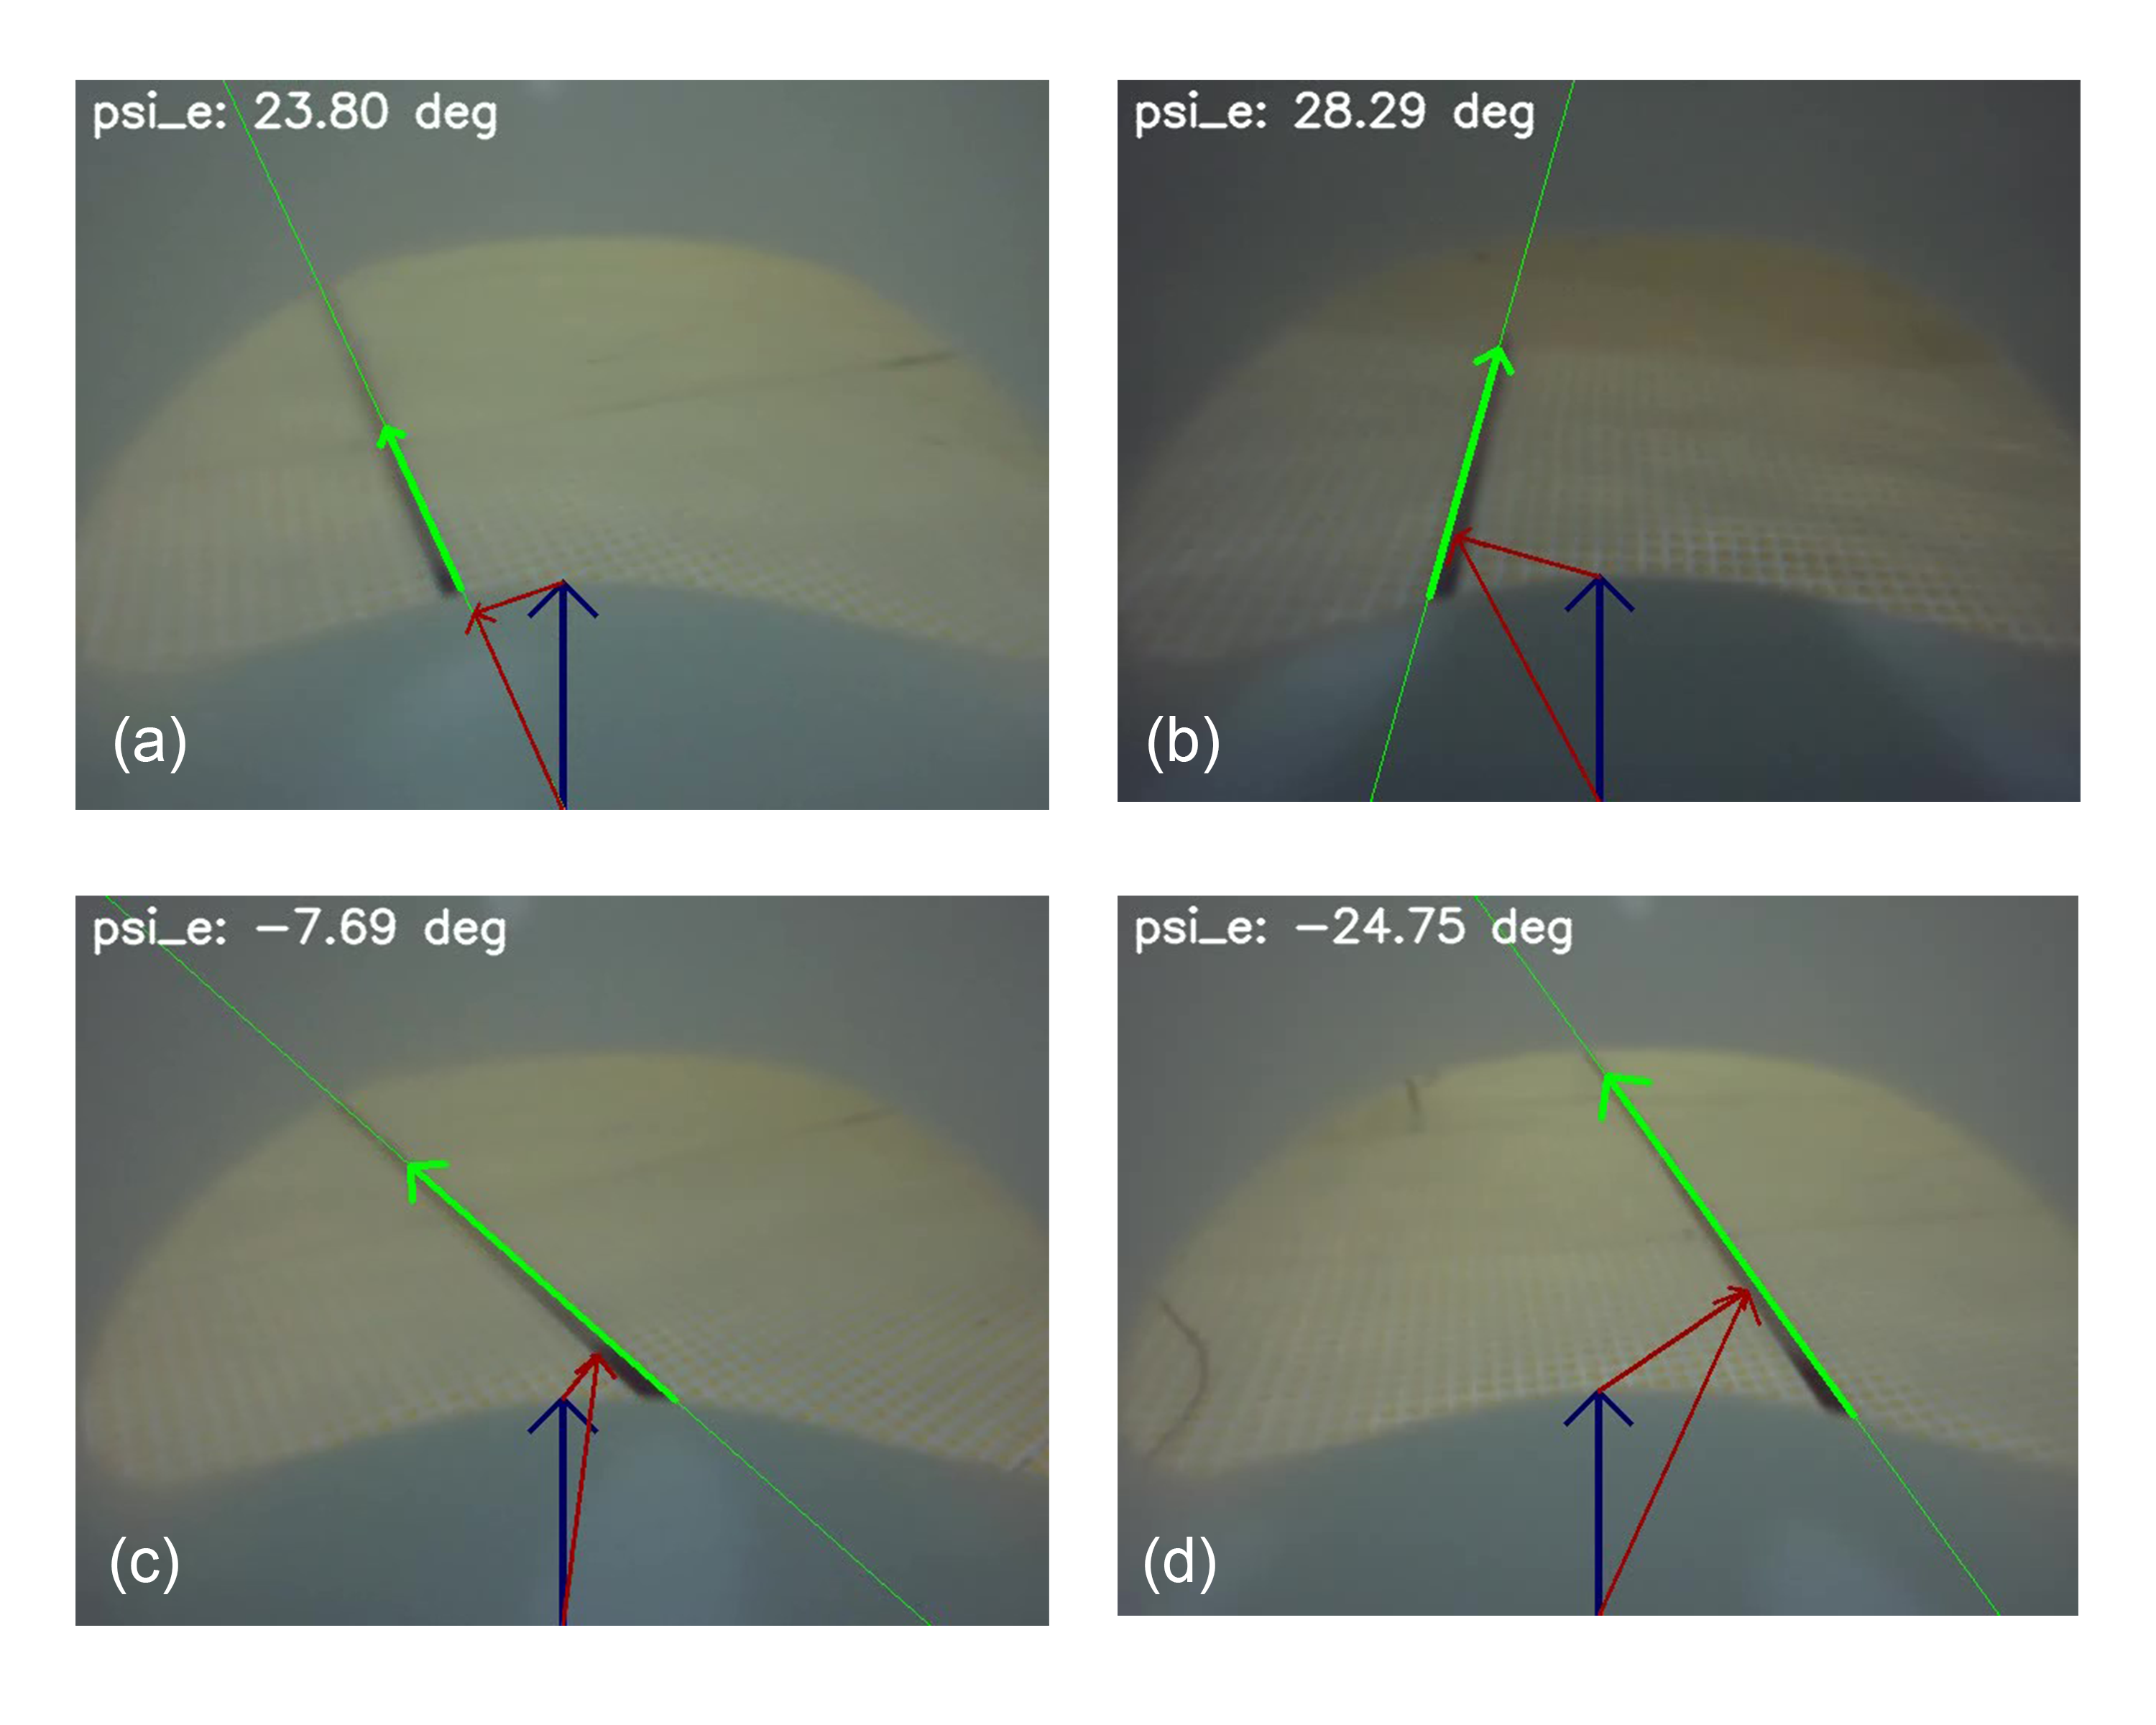
\includegraphics[width = 0.8\textwidth]{Fig/Fish-pipeline-pov.png}
    \caption{Camera view of the pipeline and the control vectors with scenarios (a) on the pipeline but not aligned (b) away from pipeline and not aligned (c) away from pipeline but heading towards pipeline (d) lateral deviation with consistent heading toward target}\label{fig:pipeline_tracking_POV}
\end{figure}
\par It is important to note here, the actual value of the $\psi_e$ angle may be different for PBVS and IBVS, and surely lead to different gains. The control algorithm is designed to converge the $\psi_e$ angle to zero, which would mean the robotic fish is aligned with the pipeline in the image space. For the proof-of-concept in this study, a simple proportional-integral-derivative (PID) controller is used to control the tail-bias angle of the robotic fish. The flapping frequency of the tail is kept constant and the control signal is sent to the servo motor to change the tail-bias angle. The control signal is calculated as follows:
\begin{equation}
    \delta (i + 1) = K_p \psi_e (i) + K_i \sum_{i - w_i}^{i} \psi_e(i) dt + K_d \frac{\psi_e(i) - \psi_e(i-1)}{dt},
    \label{eq:pid}
\end{equation}
where $K_p$, $K_i$ and $K_d$ are the proportional, integral and derivative gains of the controller. The differentiation is calculation discretized at the current iteration, while $w_i$ is the window for discrete integration. The simulation of the dynamic model helps to get a good estimation of the gains, but then the gains are tuned through a series of experiments to achieve the best tracking performance. The tail-bias angle has its physical limits and thus this leads us to a saturation of the control signal. This saturation was set to be $\pm 20\deg$ in the safety checks in the micro-controller. This limit corresponds to the maximum curvature the robotic fish can achieve in water. An additional experiment was conducted to determine the turning radius at this saturation limit, which was found to be approximately 3 meters. This value is crucial for estimating the minimum achievable turning radius during pipeline tracking tasks. The simulation environment helps to understand the performance of the controller selected, gains tuning and also the visual servoing technique selected.
\subsection{Simulation Results}
\par The simulation environment was set up with one robotic fish with parameters mentioned in Table \ref{tab:exp_vals}, and the water tank dimensions were set to $10$ m long and $5$ m wide, with a pipeline on the bottom surface of the water tank. The simulation was run for $35$ seconds with a time step of $0.05$ seconds. While pipeline being the middle of the tank, the robotic fish starting position was set to be $0.5$ m away from the pipeline and set to tail beat frequency of $11 radians/sec$ while the control signal calculated using eq. \ref{eq:pid} is updated in each iteration.
\par The tail beat propulsion is a highly efficient method when compared to traditional DC motor based thrusters in ROVs, but this introduces shaking in the body of the robotic fish. With the head movement, the camera image shakes introducing high frequency noise in the pipeline detection. As the dynamic model covers all aspects of the robotic fish, this shaking is visible in the simulation results as well. 
\par Given a sampling interval of \( \Delta t = 0.05\,\text{s} \), the system operates at a sampling frequency of \( f_s = 20\,\text{Hz} \). To suppress the high-frequency noise introduced by tail-beat-induced body shaking, a moving average filter with a window size of 15 samples is applied to error angle \( \psi_e \). This corresponds to a smoothing window of 0.75 seconds and a \(-3\,\text{dB}\) cutoff frequency of approximately \( f_c = \frac{f_s}{2N} = 0.67\,\text{Hz} \). Most of the experiments and the simulation results shown in this paper, are conducted at $\omega = 11 rads^{-1}$ which translates to $1.75 Hz$, which would be suppressed by $-13.7db$ by the designed filter.Consequently, using the filtered \( \psi_e \) for control computation effectively isolates the low-frequency components associated with true heading deviations, reducing the impact of visual noise in pipeline detection and stabilizing the closed-loop response.
\subsubsection{PBVS vs IBVS}
\par Position-based visual servoing (PBVS) requires the position of the robot relative to the target to be known in the world coordinates. In many applications, this is already known and part of the whole system, e.g. swarming robots, auto landing of a drone, etc. The PBVS is not robust to uncertainties in the camera intrinsic parameters, and calibration. Meanwhile, considering the pre-requisite is met, the PBVS is accurate and fast, of course depending upon the accuracy of 3D localization etc. 
\par The image-based visual servoing (IBVS) is more robust towards any uncertainties in the camera intrinsic, and 3D localization of the pipeline in world coordinates is not necessary. In many cases, the IBVS cannot be implemented as the image may not have a direct correlation with the world coordinates. In those cases, there needs to be some extra sensors to provide localization, thus world coordinates, and PBVS can be implemented. Meanwhile, if possible, IBVS can be computationally less expensive and faster, as the image processing is done in 2D space and the control signal is calculated in 2D space. \par Fig.~\ref{fig:pbvs} and Fig.~\ref{fig:ibvs} show the simulation results for both PBVS and IBVS, respectively. For different simulations, the $\psi_e$ angle calculated are different, but the control signal is calculated using the same PID controller with different gains. The figures show that both techniques are able to converge the $\psi_e$ angle to zero, in alsmost similar time, but this does not mean that the same gains of PID would give same tracking performance in both techniques, as the interpretation of the angle is different in both cases. In the case of underwater pipeline tracking, where the pipeline consistently appears as a straight line in the camera view when the robotic fish is aligned with it, IBVS becomes a computationally efficient and practically viable solution. As the control operates in 2D image space, both perception and control computation are significantly simplified without a substantial trade-off in performance. IBVS would also support the idea that this system can be implemented on a low-cost microcontroller with limited computational resources, making it suitable for real-world applications.
\begin{figure}
    \centering
    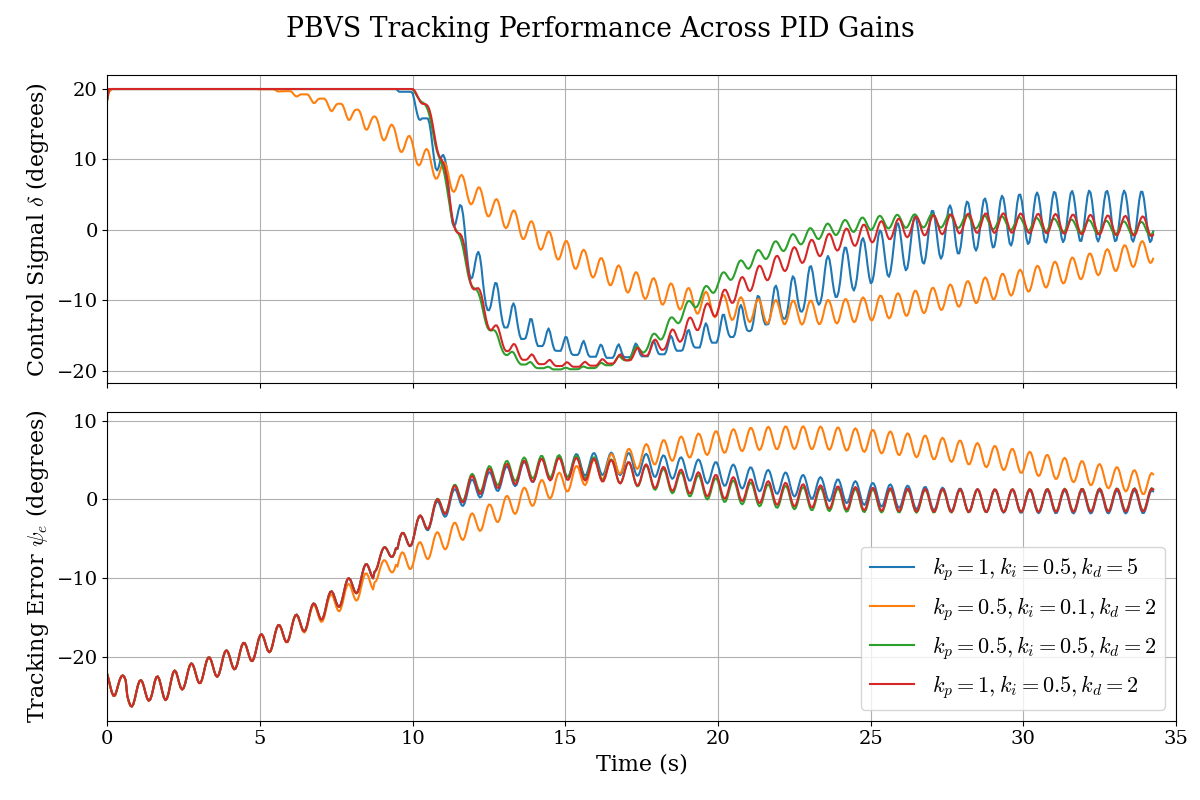
\includegraphics[width = 0.75\textwidth]{Fig/pbvs_pid.png}
    \caption{PBVS simulation tracking performance and control signal, comparison at different gains with detect vector length of $1m$.}
    \label{fig:pbvs}
\end{figure}
\begin{figure}
    \centering
    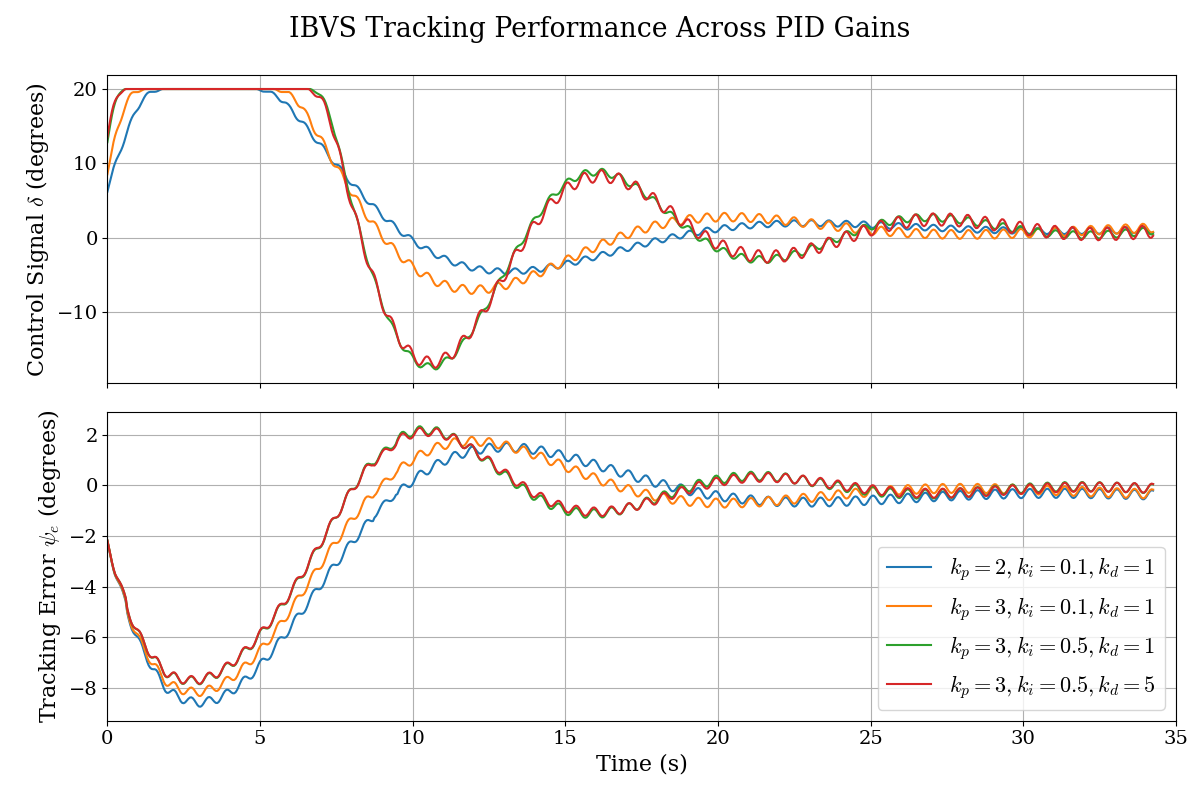
\includegraphics[width = 0.75\textwidth]{Fig/ibvs_pid.png}
    \caption{IBVS simulation tracking performance and control signal, comparison at different gains with detect vector length of $200$ pixels.}
    \label{fig:ibvs}
\end{figure}
\section{Experimental Validation}\label{experimental}
\par Experimental validation is presented in this section, which includes the design and fabrication of the robot, its operation scheme, and the experimental setup required to estimate the dynamic model parameters and validate the control performance of the proposed controller.

\subsection{Fabrication}
\par The designed parts for the AquaNavigator are fabricated using a Stereolithography (SLA) 3D printer by FormLabs\texttrademark{} and then assembled. The complete fabricated and assembled AquaNavigator is shown in Fig.~\ref{fig:fish_real} swimming in the indoor swimming pool with fresh water.
\begin{figure}[hpt]
    \centering
    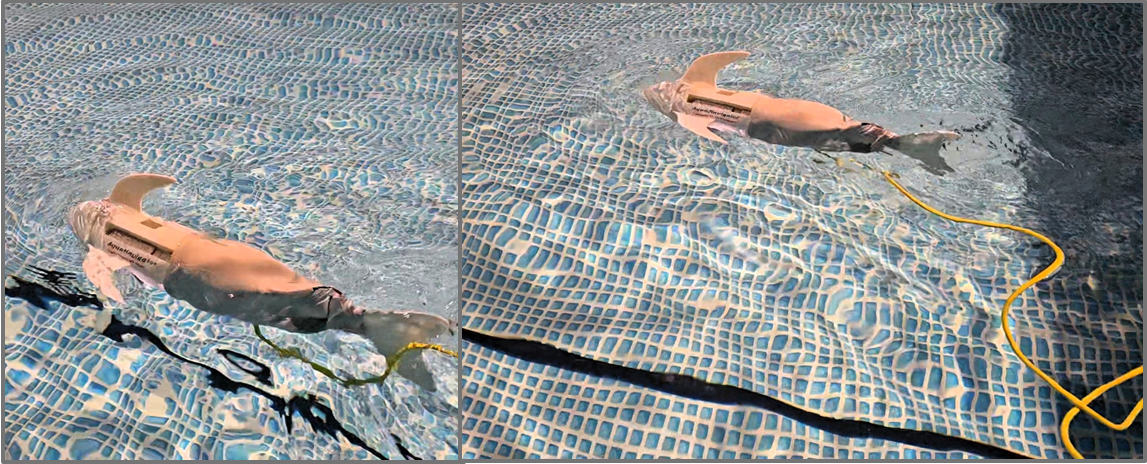
\includegraphics[width=\linewidth]{Fig/Robot_Fish_Real.png}
    \caption{Fabricated AquaNavigator swimming in a swimming pool.}
    \label{fig:fish_real}
\end{figure}
\subsection{Experimental Setup}
An indoor portable water tank, $10 m$ long and $5 m$ wide, is set up for experiments. A roof-mounted camera captures the robotic fish's motion from a top view for post-experiment analysis but does not serve as a localization device in this study.
\par The robot connects to a host computer via USB, with an onboard USB hub splitting connections between the onboard camera and microcontroller. A custom PCB integrates the power circuitry, motor drivers, microcontroller, and connectors. Powered by a 1500 mAh 3S LiPo battery, the microcontroller handles low-level commands, safety features, and actuator control, ensuring safe operation even during communication loss. All high-level commands are generated on the host computer. The host computer, running a Python-based GUI, operates the robot manually or configures pipeline tracking missions. The GUI allows adjustment of parameters like propulsion speed, Hough Transform threshold, and camera frame saving while displaying real-time camera feed, control vectors, and debugging signals, such as the servo motor's tail bias angle. Depth control is inactive, focusing solely on pipeline tracking performance. The GUI is shown in Fig.~\ref{GUI}.
\begin{figure}[hpt]
    \centering
    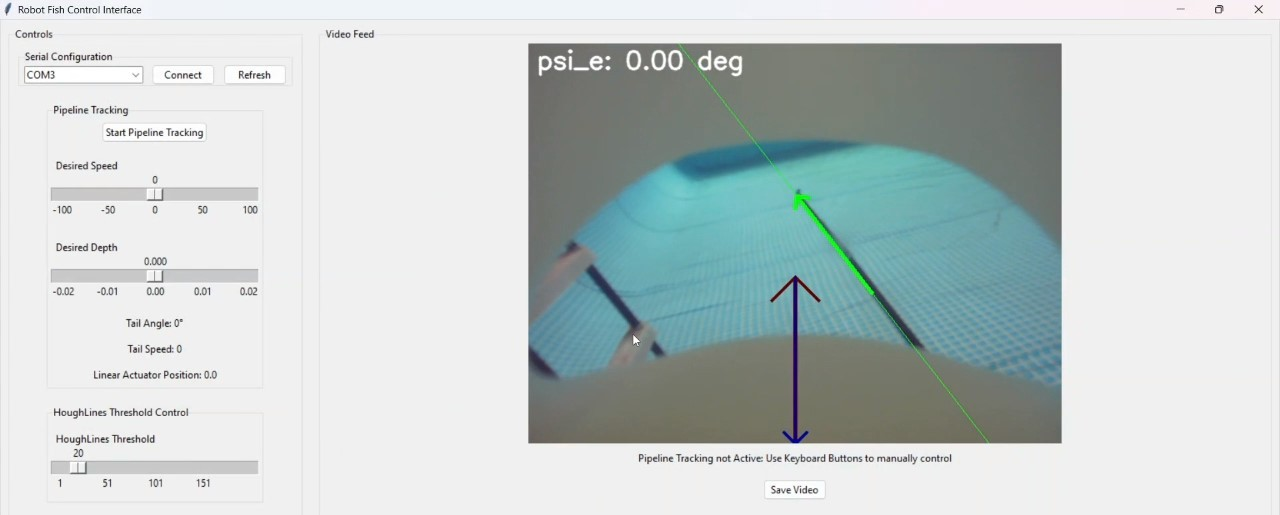
\includegraphics[width = \linewidth]{Fig/with no Image Enchancement Pipeline detected.jpg}
    \caption{Graphical User Interface for the AquaNavigator}\label{GUI}
\end{figure}
\par In the Python application, the OpenCV functions are used convert the image to grayscale, apply Canny edge detection, and Hough transform to detect the lines in the image, while the most prominent line being the pipeline. The lines are plotted on the image frame for the detected pipeline, $\vec{h_c}$, and the angle $\psi_e$. The control signal is calculated based on this angle and sent to the onboard microcontroller which applies it to the servo motor for bias angle $\delta$. After each experiment, the data is saved in a \texttt{.csv} file for post-experiment analysis. 
\subsection{Experimental Results and Discussion}\label{results}
The tracking performance is evaluated in terms of the error in the heading angle $\psi_e$ and the normal distance from the pipeline in the image frame denoted as $y$. The tracking performance along with the control signal based on the feedback control law (tail-bias angle $u$) is shown in Figure.\ref{fig:pipeline_tracking_results}. The $\psi_e$ angle is the performance parameter for the tracking, as it ensures the robotic fish is aligned with the pipeline and moving in the right direction. The normal distance is another performance parameter that provides an essence of how close the robotic fish is to the pipeline. From the plot of $y$ it is evident that the tracking started, with the robotic fish located at a distance from the pipeline. Though the robotic fish was aligned with the pipeline, as it is away, the $\psi_e$ angle it creates is about $25 \deg$. The graph shows how the $\psi_e$ angle converges to zero and eventually, the robotic fish keeps track of the pipeline. Fig.~\ref{fig:pipeline_tracking_top_camera} shows the top camera view, frame-by-frame how the robotic fish converges to the pipeline. Fig.~\ref{fig:pipeline_tracking_POV} shows the point of view of the robotic fish, how it sees the pipeline, and how it moves towards it. The control signal is saturated at $\pm 20\deg$ as discussed earlier. 
\begin{figure}[htbp]
    \centering
    \subfloat[$\psi_e$ angle in the image frame]{%
        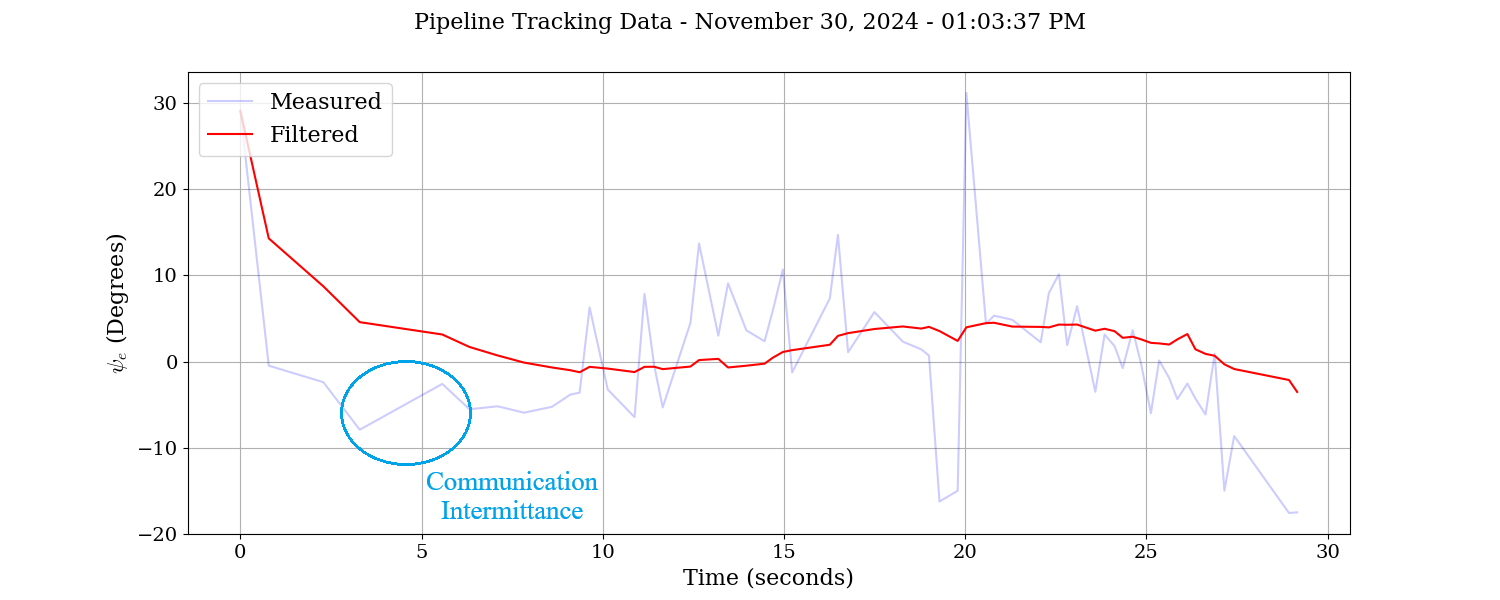
\includegraphics[width=\textwidth]{Fig/pipeline_tracking_plot_20241130_130337_psie_marked.png}\label{fig:subfig1}
    }
    \hfill
    \subfloat[Normal distance from the pipeline]{%
        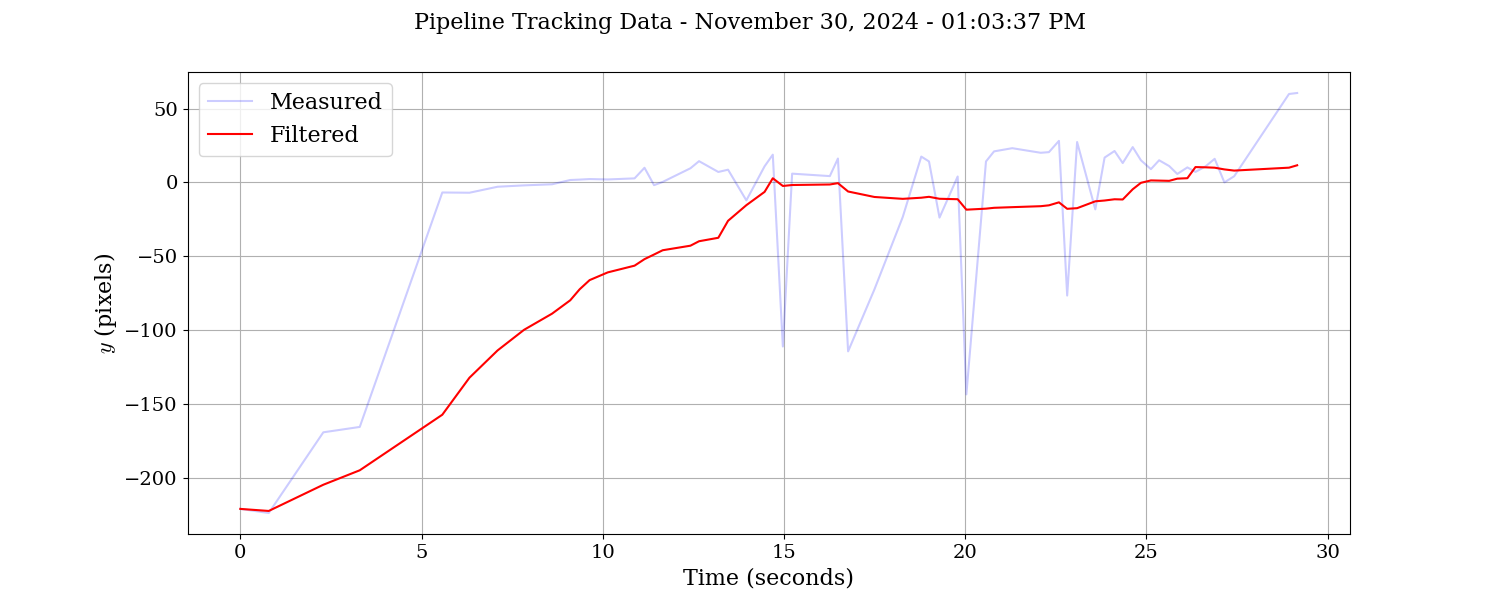
\includegraphics[width=\textwidth]{Fig/pipeline_tracking_plot_20241130_130337_y.png}\label{fig:subfig2}
    }

    \subfloat[Control signal]{%
        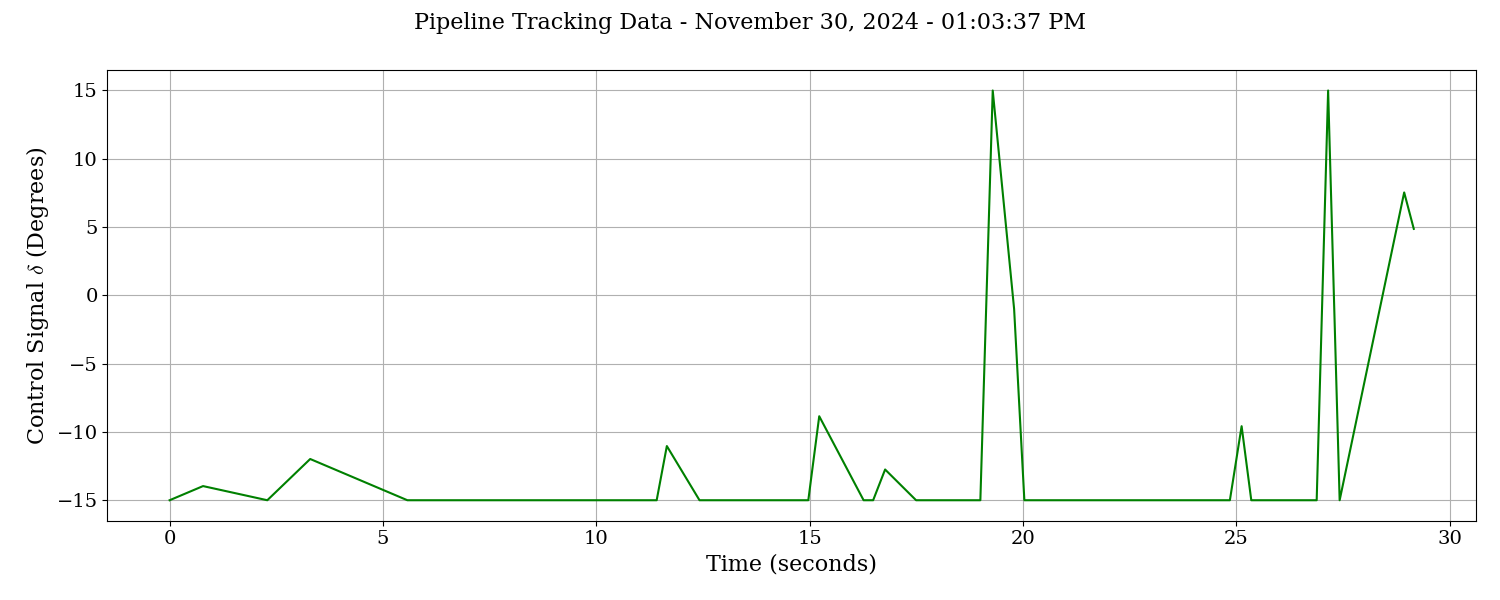
\includegraphics[width=\textwidth]{Fig/pipeline_tracking_plot_20241130_130337_u.png}\label{fig:subfig3}
    }
    \caption{Pipeline tracking experimental results plotted versus time}\label{fig:pipeline_tracking_results}
\end{figure}
\par As the robotic fish propulsion is designed based on the undulatory motion, and the mass density of the robotic fish is in the middle, unlike the oscillatory propulsion tail mechanism which focuses on the motion of a compliant tail and most of the mass is in the body. As the tail mechanism creates the undulatory motion in the tail, it naturally propagates to the complete body of the robotic fish, which creates a higher propulsion than the oscillatory tail mechanism. This oscillation of the head and body, while being useful and more naturally aspired, brings a challenge in getting stable data from the image. As evident in Fig.~\ref{fig:pipeline_tracking_results}, the actual $\psi_e$ angle acquired by the image processing is not smooth. This is because even if the robotic fish is heading in a mean direction of, say $\vec{h}$, the camera image will be shaking up to a specific extent depending on the excitation frequency of the tail mechanism.
\par This is a realistic challenge and similar to what robotic fish may see in a real ocean environment with currents. Additionally, the communication challenges and other uninvited uncertainties have to be taken care of in the real application. For this purpose, many safety features are integrated into the software, as follows:
\begin{enumerate}
    \item The robotic fish is programmed to stop the tracking and come to the surface if the pipeline is lost for more than 5 seconds.
    \item The robotic fish is programmed to turn off all the actuators and come to the surface if communication with the host computer is lost.
    \item It is experienced that the communication packet is sometimes lost, and the robotic fish is programmed to initiate a connection routine in that case.
    \item The image frame sometimes gets corrupted, leading to a wrong pipeline detection. Multiple checks are programmed to ensure the frame is legit, before proceeding to the pipeline detection routine. In the results, one can note that the robotic fish lost the connection from time stamp \( 3\,\text{s} \) to \( 6\,\text{s} \), but it was still able to continue its operation until the connection was back.
\end{enumerate}
\begin{figure*}[hpt]
    \centering
    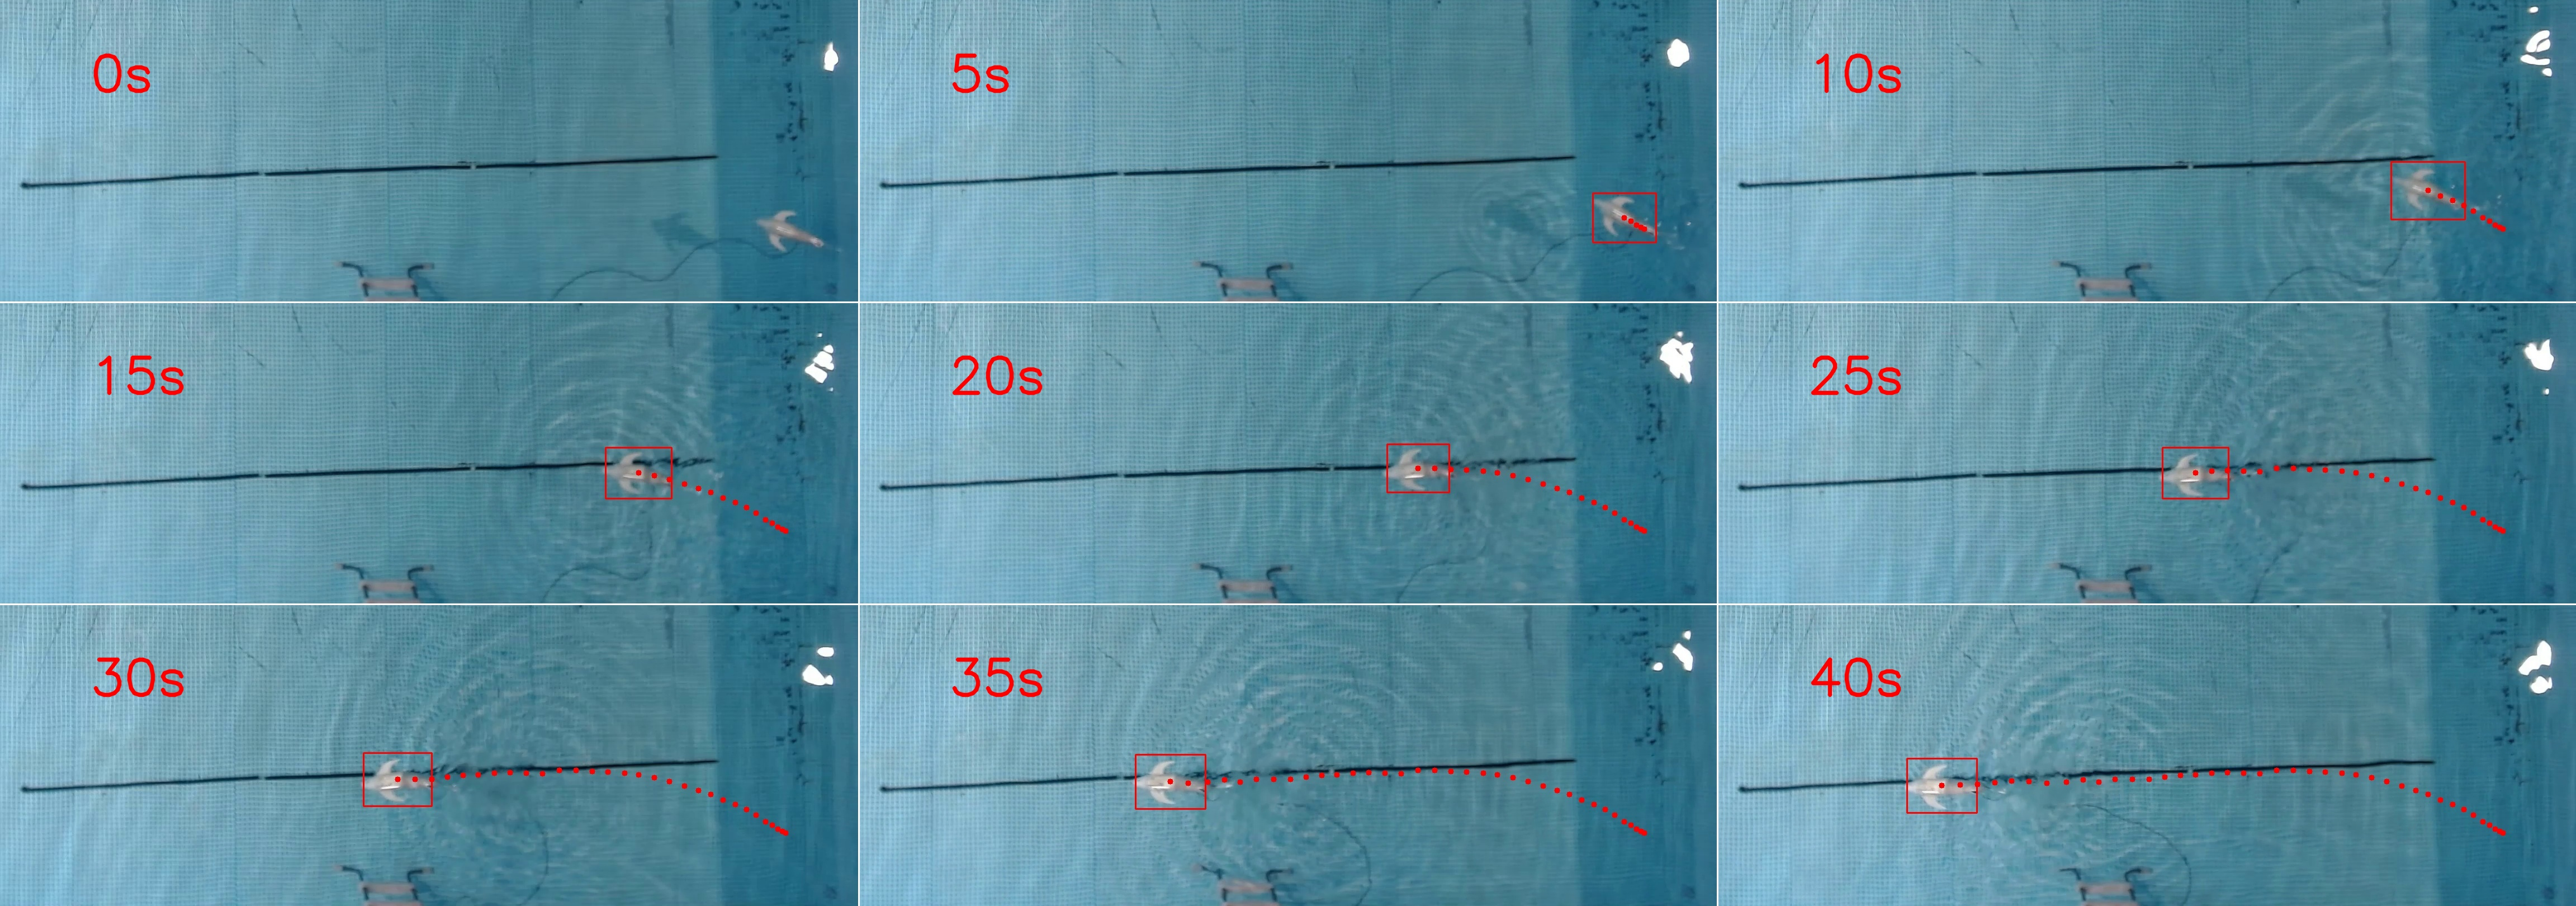
\includegraphics[width=\textwidth]{Fig/collage_topvideo_20240610_173403.jpg}
    \caption{Top camera view of the pipeline tracking}
    \label{fig:pipeline_tracking_top_camera}
\end{figure*}
Fig.~\ref{fig:pipeline_tracking_top_camera} shows the top camera view of the pipeline tracking results of Experiment 6 in Table~\ref{tab:test_results}. The robotic fish is moving towards the pipeline and eventually aligns with it and continues moving on the pipeline with steady heading velocity.
\par Multiple experiments were performed with variations of the starting point of the robotic fish scenario in terms of the orientation and location with respect to the pipeline in the image frame (starting value of $\psi_e$), and data was collected in an automated program through the Python application. For each pipeline testing experiment when conducted, the following data is stored in the \texttt{.csv} file; (1) a unique experiment ID (2) timestamp (3) $\psi_e$, and (4) $y$. The summary of some of the experiments is provided in Table \ref{tab:test_results}. Despite many physical challenges, the robotic fish is capable of tracking the pipeline and converging to within $\psi_e = \pm 5 deg$ range of the pipeline. Worth mentioning that, in Experiment 6 the starting orientation is already almost aligned with the pipeline, so the settling time is noted when the robotic fish aligned back to the pipeline after a small deviation. The settling time $(t_s)$ is noted as the time taken by the robotic fish to converge to the desired range of $\psi_e = \pm 5 deg$.
\begin{table}[h]
    \centering
    \begin{tabular}[width=\linewidth]{cccccc}
        \toprule
        Test & Span (s) & Start $\psi_e$ (deg) & Start $y$ (Pixels) & $t_s$ (s) \\
        \midrule
        1  & 11 & 28 & -3 & 11 \\
        2  & 65 & 25 & 180 & 20 \\
        3  & 45 & 22 & 175 & 9 \\
        4  & 28 & 45 & -220 & 28 \\
        5  & 15 & -25 & 130 & 7 \\
        6  & 37 & -5 & 200 & 25 \\
        \bottomrule
        \vspace{1em}
    \end{tabular}
    \caption{Test Results}
    \label{tab:test_results}
\end{table}
\section{Conclusion and Future Work}\label{conclusion}
This paper presents the design, development, and control of a 3D robotic fish, AquaNavigator, for underwater pipeline tracking. The robotic fish is designed to mimic the undulatory locomotion of biological fish, which provides a more efficient and eco-friendly solution for underwater exploration. The robotic fish is equipped with an onboard camera for vision-based tracking of underwater pipelines. The visual servoing control scheme is implemented to track the pipeline in the image space. A framework for Position-based and Image-based visual servoing is shown along with a simulator design to design the controller and validate results before pushing the robot into the water. The experimental validation shows the successful tracking of the pipeline by the robotic fish. The tracking performance is evaluated in terms of the error in the heading angle and the normal distance from the pipeline. The results show that the robotic fish can effectively track the pipeline and move in the desired direction.
\par In this paper, the robotic fish control is developed for the surface movement only, though it consists of the buoyancy control mechanism for depth adjustment. Future work will be focused on 3D motion control of robotic fish for pipeline tracking, in which the robotic fish will be able to change its depth while tracking the pipeline. To enable chemical leakage detection, chemical sensors, such as ${\rm CO_2}$ sensor will be installed on robotic fish to monitor ${\rm CO_2}$ concentration along a ${\rm CO_2}$ pipeline.
\section*{Acknowledgment}
This research is supported by Texas Commission on Environmental Quality through Subsea Systems Institute Award \#582-21-10565. This project was paid for [in part] with federal funding from the Department of the Treasury through the State of Texas under the Resources and Ecosystems Sustainability, Tourist Opportunities, and Revived Economies of the Gulf Coast States Act of 2012 (RESTORE Act).  The content, statements, findings, opinions, conclusions, and recommendations are those of the author(s) and do not necessarily reflect the views of the State of Texas or the Treasury.
\bibliography{bibliography}
\end{document}